\documentclass[12pt, letterpaper]{article}
\usepackage{amsmath, amssymb, mathtools, graphicx, listings, color, xcolor, bold-extra, tikz, tikz-qtree, colortbl, hyperref}
\usepackage[margin = 1.5in]{geometry}
\graphicspath{ {/} }

\topmargin 0in
\headheight 0in

\setlength{\parindent}{0pt}

\definecolor{codegreencomment}{HTML}{629755}
\definecolor{codegreen}{HTML}{6A8759}
\definecolor{codegray}{rgb}{0.5,0.5,0.5}
\definecolor{backcolour}{rgb}{0.95,0.95,0.92}
 
\lstdefinestyle{mystyle}{
    backgroundcolor=\color{backcolour},   
    commentstyle=\color{codegreencomment},
    keywordstyle=\color{orange}\bfseries,
    numberstyle=\tiny\color{codegray},
    stringstyle=\color{codegreen},
    basicstyle=\footnotesize\ttfamily,
    breakatwhitespace=false,         
    breaklines=true,                 
    captionpos=b,                    
    keepspaces=true,                 
    numbers=left,                    
    numbersep=5pt,                  
    showspaces=false,                
    showstringspaces=false,
    showtabs=false,                  
    tabsize=2,
    language=Scala
}
 
\lstset{style=mystyle}

\hypersetup{
    colorlinks,
    citecolor=black,
    filecolor=black,
    linkcolor=black,
    urlcolor=black
}

\usetikzlibrary{automata, positioning, calc, shapes.multipart, chains,arrows}

\begin{document}
\title{CS 241E: Foundations of Sequential Programs (Enriched)}
\author{Muhammad Talha, taught by Ondrej Lhotak }
\date{Fall 2017}

\maketitle

\tableofcontents

\newpage

\section{Machine Language}
Every instruction that the computer executes is a 32 or 64 bit binary number. An instruction that is represented by a sequence of bits is called a machine language instruction.

\subsection{Binary numbers}
In a binary number each bit is a power of 2. A binary number can be unsigned or signed.

\subsubsection{Unsigned Binary numbers}
Unsigned binary numbers are used to represent non-negative numbers. \\

E.g. Consider the following binary number:

\[
\underbrace{
\begin{tabular}{c c c c c c c}
	1 & 0 & 0 & 0 & 0 & 1 & 1 \\
	$2^6$ & $2^5$ & $2^4$ & $2^3$ & $2^2$ & $2^1$ & $2^0$
\end{tabular}
}_\text{1 + 2 + 64 = 67}
\]\\

In order to encode a number \(n\) as a binary number we need to continually find a power of 2 that is \(\leq n\).\\

E.g. Convert 42 to binary.

The highest power of 2 that is at most 42 is \(2^5 = 32\).
The highest power of 2 that is at most \(42 - 32 = 10\) is \(2^3 = 8\).
The highest power of 2 that is at most \(10 - 8 = 2\) is \(2^1 = 2\).
So the answer is \(1 0 1 0 1 0\).\\

Suppose we have 32 bits. What is the range of unsigned binary numbers? \(0\) to \(2^{32} - 1\).
In general, if we had n bits, the maximum number we can store is \(2^n - 1\).

\subsubsection{Signed binary numbers}
Signed binary numbers are used to represent negative numbers. A common format for encoding signed numbers is using 2's complement. To interpret a binary number as a 2's complement number, make the most significant bit negative.\\

E.g. \(100111 = 1 + 2 + 4 - 32 = -25\)

E.g. \(010101 = 1 + 4 + 16 = 21\)\\

Suppose we have 32 bits. What is the range of signed binary numbers?

What is the lowest number that we can store in 32 bits using 2's complement?

\[
\underbrace{
\begin{tabular}{c c c c c}
	1 & 0 & 0 & ... & 0
\end{tabular}
}_\text{$-2^{31}$}
\]\\

What is the largest number that we can store in 32 bits using 2's complement?

\[
\underbrace{
\begin{tabular}{c c c c c}
	0 & 1 & 1 & ... & 1
\end{tabular}
}_\text{$2^{31} - 1$}
\]\\

So the range of signed 2's complement numbers is: \(-2^{31}\) to \(2^{31} - 1\).\\

How do we encode a negative number using 2's complement? It turns out there is an algorithm to do this. To encode -n:

\begin{enumerate}
\item Encode n (making sure the most significant bit is 0, to indicate a non-negative number).
\item Flip all bits.
\item Add 1.
\end{enumerate}

Why does this algorithm work? Lets take a look and see what is happening step by step.

\begin{enumerate}
\item n
\item \(1 1 1 ... 1 - n = 2^{32} - 1 - n\) 
\item \(2^{32} - n \equiv -n\) mod \(2^{32}\) 
\end{enumerate}

So we see that the resulting number is congruent to \(-n\) mod \(2^{32}\). Therefore the resulting number has the same bit representation as \(-n\) in 32 bits. In general, if \(x \equiv y\) mod \(2^{32}\), then \(x\) and \(y\) have the same bit representation in 32 bits.\\

E.g. Encode -72.
\[-72 \xrightarrow{\text{encode 72}} 01001000 \xrightarrow{\text{flip all bits}} 10110111 \xrightarrow{\text{add 1}} 10111000 = -72\]

\section{Computers and Assembly Language}
A computer consists of registers and memory. Operations involving registers are efficient because they are close to the arithmetic and logic unit. Operations involving memory are slower because we first need to fetch the data from memory to registers and then do the operation.

\subsubsection{MIPS}
In MIPS there are 32 general purpose registers. Register 0 is always hard coded to store 0. Program Counter (PC) holds the address of the next instruction to execute. LO holds the quotient of a division and the first 32 bit result of a multiplication. HI holds the remainder of a division and the last 32 bits of a multiplication.\\

In MIPS, memory is indexed by multiples of 4. The first memory location is 0, the next memory location is 4 and so on.

\subsubsection{Control Unit and Step function}
The control unit of a computer is a bunch of hardware that implements a step function. A step function goes from one state of a program to the next. A state of a program is a "snapshot" that is used to represent all the bits in the computer.\\

Suppose we wanted to design a step function. We could make it specific to the task were trying to solve (make step function integrate or do algebra). The problem with that is if we make the step function too specific, it will not be able to do a wide variety of tasks. We want the step function to be as general as possible.\\

The step function that people ended up using is the following:
\begin{enumerate}
\item Fetch next instruction to execute by looking at PC.
\item Increment PC by 4.
\item Execute instruction.
\end{enumerate}

\subsubsection{Assembly}
Recall that computers only execute machine language. The problem is that it's very difficult for humans to understand machine language (i.e. interpret a bunch of bits). That is why we invented assembly language.\\

Assembly language is a language for writing machine language programs using op codes instead of sequences of bits. An op code is a word that represents a machine language instruction (e.g. ADD, SUB).\\

Note that assembly language is an \emph{abstraction} of machine language since each op code represents a machine language instruction. It's important to understand that the computer does not "see" assembly language. We need to somehow translate assembly language programs to machine language programs so that the computer can successfully execute it. The assembler is a program that translates assembly language to machine language. 

\subsubsection{Labels}
E.g. Consider the following assembly language code to find the absolute value of Reg 1:
\begin{verbatim}
	SLT $2, $1, $0
	BEQ $2, $0, 1
	SUB $1, $0, $1
	JR  $31
\end{verbatim}

Suppose we add some code between the BEQ and JR instructions. Then the BEQ jump offset would be incorrect. We have to be very careful to get the offset exactly right, otherwise we will jump to some random point in our program. The problem is that it's tedious to always update all the jump offsets in our program whenever we edit the code. Lets instead use labels.\\

A label is an abstraction of a memory address, that is, every label represents a memory address. We want to be able to define labels in memory and then jump to them.\\

E.g. Previous example with labels:
\begin{verbatim}
	SLT $2, $1, $0
	BEQ $2, $0, label
	SUB $1, $0, $1
	Define(label)
	JR  $31
\end{verbatim}

How can we compile assembly language programs with labels to just assembly language programs? We will use a symbol table. A symbol table is a map that maps labels to memory addresses they point to. Now, to eliminate labels we need to:

\begin{enumerate}
\item Go through the entire code and store each label's respective memory address in the symbol table.
\item Go through the entire code again and convert each label to an address/offset.
\end{enumerate}

Question: How do we branch to a procedure? What we can do is define a label in the beginning of the procedure. Then we can load the address of that label into a register and branch to it.\\

E.g. Calling a procedure:
\begin{verbatim}
	LIS $1
	Use(label)
	JALR(label)
	..
	Define(label)
	..procedure..
	JR  $31
\end{verbatim}

Note that instructions like Define only exist in our "intermediate language". The compiler uses them to determine addresses/offsets and removes them from the program. The compiler also does this to other instructions like comments.

\subsubsection{Relocation}
Suppose we have a block of code located at some memory address. We want this block of code to be relocatable. That is, we want to be able to take that code and place it somewhere else in memory and still be able to run exactly the same.\\

Is this possible with machine language? Suppose our code has a BEQ jumping to another part of the program (for example, BEQ \$0 \$0 104). When we relocate our code to another memory location, the address is incorrect. Therefore, it is simply not possible to relocate machine code.\\

As a result, the assembler translates assembly language files to object files. An object file is a file that contains the compiled machine language code + extra meta data. This meta data includes information regarding where the labels in the assembly file used to be and which memory locations contain addresses to other memory locations (to differentiate between a memory address and a constant). The assembler translates all assembly language files to object files and then the linker links them into a single object file.\\

However, the linker needs to relocate all the code and still make it work in the combined object file. The linker performs relocation when it links all object files. Note that the job of the linker can be done in a much easier way. Instead of linking object files, we could simply link assembly files together and make the assembler turn that into a single object file. The result would be exactly the same. So why don't we do this?\\

The reason why is modular code. Suppose we have a large project and we need to edit parts of our code. If we linked assembly files, we would have to edit the specific assembly file and compile it all again.\\

If we linked object files, all we would have to do is translate the edited assembly file to an object file and link it with the rest of the object files, thus saving time from recompiling the whole program. \\

E.g. Consider the following code snippets. The assembler will turn both files into object files and then the linker will link both files.\\

\begin{minipage}[t]{0.5\textwidth}
\emph{1.asm}
\begin{verbatim}
LIS  $1
Use(a)
JALR $1
JR   $31
\end{verbatim}
\end{minipage}
\begin{minipage}[t]{0.5\textwidth}
\emph{1.o}
\begin{verbatim}
0  LIS  $1
4  ??
8  JALR $1
12 JR   $31
Metadata:
Use imported label a @ address 4
\end{verbatim}
\end{minipage}

\vspace{5mm}

\begin{minipage}[t]{0.5\textwidth}
\emph{2.asm}
\begin{verbatim}
Define(a)
LIS $1
Use(b)
JALR $1
JR $31
Define(b)
JR $31
\end{verbatim}
\end{minipage}
\begin{minipage}[t]{0.5\textwidth}
\emph{2.o}
\begin{verbatim}
0  LIS  $1
4  16
8  JALR $1
12 JR   $31
16 JR   $31
Metadata:
export label a = 0 -> 16
export label b = 16 -> 36
Address at 4 -> 20
\end{verbatim}
\end{minipage}\\

\vspace{7mm}

In general, the assembler translates:
\begin{itemize}
\item Define(a) to \verb|export label a = ..|
\item Use(a) where a is found to \verb|Address at ..|
\item Use(a) where a is not found to \verb|use imported label a @ address ..|
\end{itemize}

Now lets link the two object files together:

\begin{verbatim}
0  LIS  $1
4  ?? -> 16
8  JALR $1
12 JR   $31
16 LIS  $1
20 16 -> 32
24 JALR $1
28 JR   $31
32 JR   $31
\end{verbatim}

The first to note is that the file \emph{1.o} and \emph{2.o} start at memory address 0. However, in the linked program, \emph{2.o} starts at 16 since the size of \emph{1.o} is 16.\\

This is a problem because all of the second file's meta data is off by an offset of 16. So we need to perform relocation on the second file's meta data.\\

We read the first file's meta data and see at address 4 we need to use imported label a. So lets set address 4 to be a. We read the second file's meta data and see there is an address at 20. The problem is that any address value is also going to be off by an offset of 16. So lets add 16 to the address value. Thus we get the resulting correct object file.

\section{Variables}
Variables are abstractions of memory addresses that can be used in expressions. Variables are very useful as we can simply store any value we want in them. There are two types of variables: global variables and function local variables.\\

Global variables are accessible from anywhere and anytime in the program.

Function local variables are accessible only during function execution.\\

The extent of a variable is the time interval in which its value can be accessed. For global variables, the extent is the entire execution of the program. For function local variables, the extent is only one execution of the function (i.e. every time a function is called a new local variable is created).

\subsubsection{Stack}
E.g. Consider the following code:
\begin{lstlisting}[mathescape]
def fact(x: Int): Int = if (x $\leq 1$) 1 else x $\cdot$ fact(x - 1)
\end{lstlisting}


Suppose we call fact(3). This would be evaluated to \(3 \times\) fact(2), \(3 \times 2 \times\) fact(1) and finally return \(3 \times 2 \times 1\). Note that there are actually 3 run time instances of the variable x. That is, x is 3 in fact(3), 2 in fact(2) and 1 in fact(1). After x is 1 in fact(1), the value 1 returns and that run time instance of x is deallocated. Then x is 2 is deallocated followed by x is 3.\\

What kind of data structure can we use that allows us to easily:

Allocate x = 3, x = 2, x = 1

Deallocate x = 1, x = 2, x = 3\\

We can use a stack. Every time we allocate a variable, we can push it onto the stack. Every time we deallocate a variable, we pop from the stack. We can implement a stack by considering a block of memory to be the stack and have a register (called stack pointer, SP) that always points to the top of stack.\\

Convention: Lets put the stack at the end of memory and use register 30 as the SP.
To push a word we need to decrement the SP by 4. To pop a word we need to increment the SP by 4.
Lets initialize the SP to point to the address one word after the end of memory. Then, when we push a word, that word will be located right at the end of memory.\\

\[
\begin{tabular}{|c|}
\hline
Code\\
\hline
1010..\\
..\\
..\\
\hline
Stack\\
\hline
x\\
\hline
\end{tabular}
\]\\

Suppose a function pushes variables a, b and c onto the stack. How can it access those variables again? One idea might be to use a symbol table mapping each variable to its offset from the SP. However, there is a problem with this idea. Suppose that same function wanted to use the stack again. It cannot simply add other things onto the stack because, if it does, the symbol table mapping each variable to its SP offset will be incorrect.\\

Lets instead use a frame. Whenever we call a function lets allocate its frame onto the stack. This frame will act as a container for all of the function's variables. Since the top of the stack and the top of the frame might not point to the same thing (i.e. function decides to use the stack again), we need another register that points to the top of the frame.\\

Convention: Lets use register 29 to point to the top of the frame (called frame pointer, FP).\\

Now, instead of the symbol table holding each variable's SP offset, it will hold each variable's FP offset. This allows the function to modify the stack \emph{and} still have access to its variables via the symbol table.\\

Convention: For CS 241E assignments, all memory is organized in chunks. The first two words of the chunk are reserved and always hold the size of the chunk and some data that will be useful for assignment 11.

\[
\begin{tabular}{|c|}
\hline
Size of chunk\\
\hline
A11\\
\hline
Variables..\\
\hline
\end{tabular}
\]\\

Now that we have figured out how to store variables, how can we use them in an expression?

\subsubsection{Expressions}
An expression is a variable or an operation involving two sub expressions (E.g. a, a + b). In order to compile expressions we need to generate code for its sub expressions.\\

E.g. Let a, b, c and d be variables. Consider the expression: \((a \cdot b) + (c \cdot d)\).\\

In order to generate code for this expression we need to first MUL a and b, store the result, and then MUL c and d, store the result, and finally ADD the two results.\\

Convention: Whenever we evaluate an expression, put the result into register 3 (Reg.result).\\

In general, how can we evaluate \(e_1\) op \(e_2\)? We cannot simply evaluate the first sub expression and then the next sub expression, as the result of the first sub expression will be overwritten. There are 3 techniques that we will study in order to evaluate expressions.

\paragraph{Technique 1: Using a Stack} \hfill

The main idea of technique 1 is saving the result of the first sub expression onto the stack. Note that push and pop correspond to the Stack push and pop.

\begin{lstlisting}[escapeinside={(*}{*)}]
def evaluate((*$e_1$*) op (*$e_2$*)): Code = block(
	evaluate((*$e_1$*)),
	push $3,
	evaluate((*$e_2$*)),
	pop $4,
	$3 = $4 op $3
)
\end{lstlisting}

E.g. How does this generate code for \((a \cdot b) + (c \cdot d)\)?

\begin{verbatim}
read a
push $3
read b
pop $4
$3 = $4 * $3
push $3
read c
push $3
read d
pop $4
$3 = $4 * $3
pop $4
$3 = $4 + $3
\end{verbatim}

What are some advantages of this technique? It is general, simple.

What are some disadvantages? Inefficient (lots of pushing and popping), difficult to optimize further.

\paragraph{Technique 2: Using Variables to save result} \hfill

The main idea of technique 2 is using variables to store the result of the two sub expressions. We will create one variable to store the result of \(e_1\), another variable to store the result of \(e_2\) and finally return the result of  \(e_1\) op \(e_2\) in a variable.\\

\begin{lstlisting}[escapeinside={(*}{*)}]
def evaluate((*$e_1$*) op (*$e_2$*)): (Code, Variable) = block(
	val ((*$c_1$*), (*$v_1$*)) = evaluate((*$e_1$*))
	val ((*$c_2$*), (*$v_2$*)) = evaluate((*$e_2$*))
	val (*$v_3$*) = new Variable
	val code = block((*$c_1$*), (*$c_2$*), ((*$v_3$*) = (*$v_1$*) op (*$v_2$*)))
	(code, (*$v_3$*))
)
\end{lstlisting}

What are some advantages of this technique? It is flexible, easy to optimize.

What are some disadvantages? Inefficient (lots of variables). Recall that the computer only performs arithmetic operations on registers. That means whenever we perform an operation like (\(v_3\) = \(v_1\) op \(v_2\)), we need to read \(v_1\) and \(v_2\) to registers, perform the operation and then write the result to \(v_3\).

\paragraph{Technique 3: Using \emph{a} Variable to save result} \hfill

The main idea of technique 3 is combining techniques 1 and 2. All we really need is one temporary variable to store the result of \(e_1\).\\

Convention: In assignments we have another abstraction called withTempVar. This abstraction is a piece of code that holds a piece of code and a temporary variable that the code uses. In order to create a withTempVar you need to pass a function that accepts a variable and returns a piece of code that uses the variable. Then withTempVar will create the temporary variable and wrap it around the code that the function returns.\\

\begin{lstlisting}[escapeinside={(*}{*)}]
def evaluate((*$e_1$*) op (*$e_2$*)): Code = withTempVar{
	(*$t$*) => block(
		evaluate((*$e_1$*)),
		write((*$t$*), $3),
		evaluate((*$e_2$*)),
		read($4, (*$t$*)),
		$3 = $4 op $3
	)
}
\end{lstlisting}

E.g. How does this generate code for \((a \cdot b) + (c \cdot d)\)?

\begin{verbatim}
read a
t_1 = $3
read b
$4 = t_1
$3 = $4 * $3
t_2 = $3
read c
t_3 = $3
read d
$4 = t_3
$3 = $4 * $3
$4 = t_2
$3 = $4 + $3
\end{verbatim}

Note that now all operations are done on registers. This technique has the perfect balance between flexibility and efficiency. We will apply this technique in the assignments.

\section{Control Structures}
We want our language to have control structures like if statements and while loops.

\subsubsection{If statements}
\begin{lstlisting}[mathescape]
if ($e_1$ op $e_2$) $\underbrace{T}_\text{thens}$ else $\underbrace{F}_\text{elses}$
\end{lstlisting}

We can implement if statements with a simple BEQ and labels.\\

\begin{lstlisting}[escapeinside={(*}{*)}]
def eliminateIfStmts(ifStmt: IfStmt): Code = withTempVar{
	t => block(
		evaluate((*$e_1$*)),
		t = $3,
		evaluate((*$e_2$*)),
		$3 = $4 op $3,
		beq($3, $0, elseLabel),
		ifStmt.thens,
		beq($0, $0, endIf),
		Define(elseLabel),
		ifStmt.elses,
		Define(endIf)
	)
}
\end{lstlisting}

Note that after executing the thens code, we need to branch to the end, otherwise we will end up executing the elses code as well.\\

\subsubsection{While loops}
\begin{lstlisting}[mathescape]
while ($e_1$ op $e_2$) $\underbrace{B}_\text{keep executing as long as exp. true}$
\end{lstlisting}

We can implement if statements with a simple BEQ and labels.\\

\begin{lstlisting}[escapeinside={(*}{*)}]
def eliminateWhile(whileLoop: WhileLoop): Code = withTempVar{
	t => block(
		Define(startWhile),
		evaluate((*$e_1$*)),
		t = $3,
		evaluate((*$e_2$*)),
		$3 = $4 op $3,
		beq($3, $0, endWhile),
		whileLoop.B,
		beq($0, $0, startWhile),
		Define(endWhile)
	)
}
\end{lstlisting}

Note that after executing the while block, we need to branch back to the beginning of the while loop to test if the condition still holds true.\\

\subsubsection{Arrays}
Arrays can be easily implemented, using a similar technique as when were implementing the stack. All we really need to do is store the start of the array. Whenever the user wants to access element i, we need to access address \(start + 4*i\). Although arrays are simple to implement, we will not be implementing them in the assignments.

\section{Register Allocation}
Suppose you have an expression containing 33 variables. Since there are only 32 registers in MIPS assembly, we cannot read every single variable into a register and perform the designated operation. Register allocation deals with the problem of mapping a large number of variables to a small number of registers.\\

E.g. Consider the following code with variables \(t_1, t_2, t_3, t_4\):
\begin{lstlisting}[mathescape]
$t_1$ = a + b
$t_2$ = $t_1$ + c
$t_3$ = $t_2$ + d
$t_4$ = $t_3$ + e
\end{lstlisting}

How many registers do we really need? Do we need 4 registers to store \(t_1, t_2, t_3, t_4\) independently? No. We know we can deal with this particular code by using just 1 register. We can put \(a\) into this register and add \(b\), \(c\), \(d\), and \(e\) to it.\\

A program point is a point between two pieces of code. It's nice to define a program point between two pieces of code as there's no ambiguity (we know every thing above the program point has already executed and every thing below the program point has not yet executed).\\

We say a variable is live at program point P if its value may be read later in the program. The live range of a variable is the set of all program points where the variable is live.\\

Notice that we only need to know variables values at program points in its live range. For example, if a program point P is not in a variables live range, then the variables value will not be read after the program point P. As a result, there's no need to store its value.\\

Two variables can share a memory address if their live ranges are disjoint. To understand this, consider two variables who have at least one program point P where both variables are live. Then, at this program point P, the first variable's value may be read later in the program \emph{and} the second variable's value may be read later in the program. Therefore, we need two memory locations to store both variable values.\\

E.g. Consider the following code in the previous example:
\begin{lstlisting}[escapeinside={(*}{*)}]
(*$t_1$*) = a + b
(*\textcolor{codegreen}{Live: $t_1$}*)
(*$t_2$*) = (*$t_1$*) + c
(*\textcolor{codegreen}{Live: $t_2$}*)
(*$t_3$*) = (*$t_2$*) + d
(*\textcolor{codegreen}{Live: $t_3$}*)
(*$t_4$*) = (*$t_3$*) + e
(*\textcolor{codegreen}{Live: $t_4$}*)
..
println((*$t_4$*))
\end{lstlisting}

We see that the live range of all \(t_i\) is disjoint with \(t_j\) (\(i \neq j\)). So we can use one register to store \(t_1, t_2, t_3, t_4\).\\

E.g. Consider the following code:
\begin{lstlisting}[escapeinside={(*}{*)}]
(*$t_1$*) = a * b
(*\textcolor{codegreen}{Live: $t_1$}*)
(*$t_2$*) = c * d
(*\textcolor{codegreen}{Live: $t_1, t_2$}*)
(*$t_3$*) = (*$t_1$*) + (*$t_2$*)
(*\textcolor{codegreen}{Live: $t_3$}*)
(*$t_4$*) = e * f
(*\textcolor{codegreen}{Live: $t_3, t_4$}*)
(*$t_5$*) = (*$t_3$*) - (*$t_4$*)
(*\textcolor{codegreen}{Live: $t_3, t_5$}*)
g = (*$t_3$*) + (*$t_5$*)
\end{lstlisting}

Notice that the live range of \(t_1\) is \(\{P_1, P_2\}\), \(t_2\) \(\{P_2\}\), \(t_3\) \(\{P_3, P_4, P_5\}\), \(t_4\) \(\{P_4\}\), \(t_5\) \(\{P_5\}\).\\

Since the live range of \(t_1\) and \(t_2\) are not disjoint, we need at least 2 registers.\\

We say a variable is dead at a program point P if it's never read after P or its value is overwritten before it's read.\\

Now that we can tell whether two or more variables can share a memory location, how do we actually map the variables to registers?\\

We will use an inference graph. The basic idea is that the vertices are variables. There exists an edge between two vertices (two variables) if both variables are live at the same time.\\

E.g. For the above example, the inference graph is:
\begin{center}
\begin{tikzpicture}
	\node[shape=circle,draw=black] (t1) at (1, 4) {$t_1$};
	\node[shape=circle,draw=black] (t2) at (4, 4) {$t_2$};
	\node[shape=circle,draw=black] (t3) at (0, 1) {$t_3$};
	\node[shape=circle,draw=black] (t5) at (5, 1) {$t_5$};
	\node[shape=circle,draw=black] (t4) at (2.5, 0) {$t_4$};

	\path [-] (t1) edge node[] {} (t2); 
	\path [-] (t3) edge node[] {} (t5); 
	\path [-] (t3) edge node[] {} (t4); 
\end{tikzpicture}
\end{center}

Now that we have an inference graph, we need a graph coloring. A graph is \(k\)-colorable if you can color all the vertices of the graph with \(k\) colors such that no two adjacent vertices have the same color.\\

The idea is that a color represents a register. We want to minimize the number of colors (registers) used. However, the problem of finding the minimal graph coloring for an arbitrary graph is NP-hard. There do exist simple greedy algorithms that do quite well but, in general, don't find the minimal graph coloring.\\

\begin{lstlisting}[escapeinside={(*}{*)}]
for (v <- vertices){
	(*color v with the lowest numbered color not yet used by its neighbours*)
}
\end{lstlisting}

E.g. For the example above:
\begin{center}
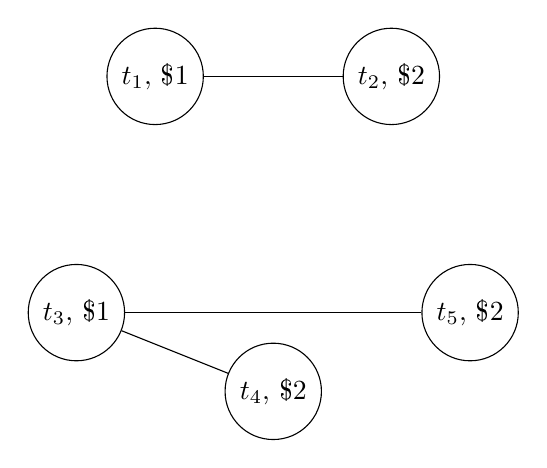
\begin{tikzpicture}
	\node[shape=circle,draw=black] (t1) at (1, 4) {$t_1,$ \$1};
	\node[shape=circle,draw=black] (t2) at (4, 4) {$t_2$, \$2};
	\node[shape=circle,draw=black] (t3) at (0, 1) {$t_3$, \$1};
	\node[shape=circle,draw=black] (t5) at (5, 1) {$t_5$, \$2};
	\node[shape=circle,draw=black] (t4) at (2.5, 0) {$t_4$, \$2};

	\path [-] (t1) edge node[] {} (t2); 
	\path [-] (t3) edge node[] {} (t5); 
	\path [-] (t3) edge node[] {} (t4); 
\end{tikzpicture}
\end{center}

So \(t_1, t_3\) would be mapped to register 1, and \(t_2, t_4, t_5\) would be mapped to register 2.
The resulting code would now look like:

\begin{lstlisting}
$1 = a * b
$2 = c * d
$1 = $1 + $2
$2 = e * f
$2 = $1 - $2
g = $1 + $2
\end{lstlisting}

If the graph coloring algorithm requires more colors than number of available registers, then we can allocate some colors to represent memory locations on the stack.\\

However, in the assignments we will allocate all variables on the stack for simplicity.

\section{Procedures}
Procedures are an abstraction of a reusable block of code. How do we implement them? Suppose a procedure, called caller procedure, calls another procedure, called callee procedure.\\

The first thing we have to do is branch to the label of the procedure. We will load the address of the callee procedure into Reg.targetPC, and branch to it.\\

\begin{minipage}[t]{0.5\textwidth}
\emph{Caller procedure}
\begin{verbatim}
LIS (Reg.targetPC)
Use(procedureLabel)
JALR(Reg.targetPC)
\end{verbatim}
\end{minipage}
\begin{minipage}[t]{0.5\textwidth}
\emph{Callee procedure}
\begin{verbatim}
Define(procedureLabel)
\end{verbatim}
\end{minipage}

\vspace{7mm}

After calling the callee procedure, the caller procedure's code needs to continue executing. 
We will use Reg.savedPC (i.e. the link register) to store the address of the next instruction to execute after calling the callee procedure. The JALR instruction does this automatically, and sets Reg.savedPC to be the value of PC and then jumps to the specified address.\\

However, there is a problem with this. Suppose the callee procedure has some code that calls another procedure. Then that call will update Reg.savedPC to be the address of the next piece of code after calling that procedure. Now, when the callee procedure returns, it will attempt to jump to the value of Reg.savedPC to return to the caller procedure. However, this will create an infinite loop.\\

We need to \emph{preserve} the value of Reg.savedPC. To do this, we will save the value of Reg.savedPC in the callee procedure's frame and then set it back to what it was before returning from the procedure. However, we first need to allocate the callee procedure's frame. Since we are allocating a new frame, we should set the FP to be the address of the top of the frame. Note that the old FP points to the caller procedure's frame and the caller procedure uses it to access it's variables. So we need to \emph{preserve} the value of Reg.FP as well.\\

Convention: We will save Reg.savedPC in a variable called savedPC and Reg.FP in a variable called dynamicLink.\\

\begin{minipage}[t]{0.5\textwidth}
\emph{Caller procedure}
\begin{verbatim}
LIS (Reg.targetPC)
Use(procedureLabel)
JALR(Reg.targetPC)
\end{verbatim}
\end{minipage}
\begin{minipage}[t]{0.5\textwidth}
\emph{Callee procedure}
\begin{verbatim}
Define(procedureLabel)
Stack.allocate(frame)
dynamicLink = Reg.FP
savedPC = Reg.savedPC
Reg.FP = Reg.allocated
..
..
Reg.savedPC = savedPC
Reg.FP = dynamicLink
Stack.pop // Pop frame
JR(Reg.savedPC)
\end{verbatim}
\end{minipage}

\vspace{7mm}
Note that while we are saving the value of Reg.savedPC and Reg.FP, we need to write to the callee procedure's frame at base offsets of Reg.allocated. The reason why is because Reg.FP currently points to the old FP.\\

Question: How do we pass parameters to the callee procedure?\\

The caller procedure should allocate a parameter chunk on the stack that will store all the computed parameters. One solution might be to have the caller allocate the parameter chunk and then store the results. However, this might be difficult to do. The solution works fine for normal expressions (E.g. f(1 + 1, 2 + 5)) but what if we call another function as a parameter (E.g. f(g())?\\

Here we will allocate a parameter chunk for f() and, while we are evaluating its parameters, we will need to call g(). This will create another parameter chunk and now we need to be careful to write to the correct parameter chunk.\\

An easier solution is to evaluate all parameters to temporary variables and then allocate a parameter chunk and write the results of those temporary variables to the newly created parameter chunk. Now that the caller procedure has created a parameter chunk, it needs to tell the callee procedure of its location.\\

Convention: The callee procedure will expect address of its parameter chunk to be stored in Reg.allocated. However, as soon as the callee procedure creates its own frame, it will overwrite the address of its parameter chunk. So we need to \emph{preserve} the address of the parameter chunk. Lets initially save it to a new register, Reg.savedParamPtr, and then store it in a variable called paramPtr.\\

\begin{minipage}[t]{0.5\textwidth}
\emph{Caller procedure}
\begin{verbatim}
evaluate params to temp vars 
Stack.allocate(paramChunk)
param1 = temp1
param2 = temp2
..
..
LIS (Reg.targetPC)
Use(procedureLabel)
JALR(Reg.targetPC)
\end{verbatim}
\end{minipage}
\begin{minipage}[t]{0.5\textwidth}
\emph{Callee procedure}
\begin{verbatim}
Define(procedureLabel)
Reg.savedParamPtr = Reg.allocated
Stack.allocate(frame)
dynamicLink = Reg.FP
savedPC = Reg.savedPC
Reg.FP = Reg.allocated
paramPtr = Reg.savedParamPtr
..
..
Reg.savedPC = savedPC
Reg.FP = dynamicLink
Stack.pop // Pop frame
Stack.pop // Pop param chunk
JR(Reg.savedPC)
\end{verbatim}
\end{minipage}

\vspace{7mm}

We call the code at the beginning of the callee procedure the prologue and the code at the end of the epilogue.\\

In general, a register is caller save if its value is not preserved by the procedure call. So if the caller wishes to preserve its value, they will need to save it. A register is callee save if its value is preserved by the procedure call. So if the callee wishes to change its value, they will need to save it and then return it back to normal.\\

Reg.FP and Reg.SP are callee save. Note that the SP is preserved because we are doing equal number of push and pops. Reg.savedPC, Reg.result and all other registers are caller save.\\

We also need to revisit the variable abstraction. Previously, we implemented the variable abstraction by writing/reading at an offset from the FP. However, now a procedure can also access variables in its parameter chunk.\\

\begin{lstlisting}
def eliminateVarAccessesA5(variable: Variable): Code = {
	if (variable is not a parameter){
		read/write at offset from FP using symbol table
	} else {
		read paramPtr from frame to Reg.scratch
		read/write at offset from Reg.scratch
	}

}
\end{lstlisting}

Note that we cannot read the paramPtr to Reg.result because it will overwrite the value of an expression during a variable assignment. For a variable assignment, \(p = exp\), the value of \(exp\) will be evaluated to Reg.result. While we are compiling the variable, if we read paramPtr into Reg.result, it will overwrite the value of the expression.

\subsubsection{Nested Procedures}
E.g. Consider the following code:
\begin{lstlisting}
def f() = {
	val w = 5
	
	def g(){
		val w = 7
		h() + 10		
	}
	
	def h(){
		20 + w
	}
	
	g()
}
\end{lstlisting}

Suppose we call f(). What does h() evaluate to, 5 or 7?\\

It turns out it can be both. A programming language either has dynamic scope or static scope.\\

Dynamic scope means when the language is evaluating variables, if a variable cannot be found in the current scope, it looks in the scope of the procedure that called it. Static scope means when a language is evaluating variables, if a variable cannot be found in the current scope, it looks in the enclosing procedure's scope.\\

If the language was dynamic scope, then w would evaluate to 7 since g() called h(). If the language was static scope, then w would evaluate to 5 since f() is h()'s enclosing procedure.\\

How would we implement dynamic scope? 

Suppose a procedure attempts to access a variable that is not found in the frame's variables or parameters. Then we need to search for the variable in the scope of the caller procedure. We can easily get access to the caller procedure's frame because it is stored in a variable in our frame, dynamicLink. So, to implement dynamic scope, we need to update the variable abstraction to continually follow the dynamicLink until the variable is found.\\

How would we implement static scope?

We need a way for every procedure to access its enclosing procedure's frame. We will use a static link. For each procedure, the static link will point to the enclosing procedure's frame. If there is no enclosing procedure (i.e. the procedure is a top level procedure), then the static link will simply point to the current procedure's frame. So, to implement static scope, we need to update the variable abstraction to continually follow the static link until the variable is found. \\

How do we find out the static link for each procedure?

Similar to passing the parameter pointer to the callee procedure, the caller procedure will pass the static link to the callee procedure during a procedure call.\\

Convention: The caller will pass the static link in the callee procedure's parameter chunk.\\

The first case we need to handle is when a procedure calls one of its direct child procedures. In this case, the static link of the callee will be the frame of the caller. For example:\\

\begin{lstlisting}
def f() = {
	def g(){}
	def h(){
		def k(){}	
	}
}
\end{lstlisting}

Suppose f() calls g(), a direct child of f(). It will pass its frame pointer to g(), which will let g() have access to its enclosing procedure's frame.\\

Now suppose a procedure does not call one of its direct child procedures. In the above example, suppose g() calls h(). Then g() has access to h()'s static link, which is just g()'s static link. Now suppose k() calls g()\footnote{How does k() get access to its own static link? h() must have called k() and passed its frame pointer as the static link. }. Then k() has access to g()'s static link, which is h()'s static link. Note that k() can access h()'s static link because it is a variable stored in h()'s parameter chunk and we updated the variable abstraction to continually follow the static link until a variable is found.\\

In both of the above cases, the caller traverses up 0 or more times to return the callee's static link. If g() calls h(), g() traverses up 0 times to return g()'s static link. If k() calls g(), k() traverses up 1 times to return h()'s static link. In general, let \(n\) be the number of times the caller needs to traverse up to return the callee's static link:

\begin{gather*}
n = depth(\text{caller procedure}) - depth(\text{callee procedure})
\end{gather*}\\

In conclusion, to implement static scope we need to do the following things:
\begin{itemize}
\item Update the variable abstraction to continually follow the static link until a variable is found
\item If a procedure is calling one of its direct children, in which case \(n\) will be equal to \(-1\), just return the caller's frame pointer
\item Otherwise, traverse up \(n\) times and return the resulting procedure's static link
\end{itemize}

It seems the values that \(n\) can take on are \(\{-1, 0, 1, 2, ..\}\). Can n take on a value \(\leq -2\)? Suppose f() calls k(). In this case, \(n = 0 - 2 = -2\). However, this call is invalid because f() should not be able to call k() without calling h() first. So n can only take values in \(\{-1, 0, 1, 2, ..\}\).

\newpage

\section{Closures}
So far we have dealt with integers in our language. That is, our language allows creating a variable and assigning a integer value to it. However, now we want to be able to create a variable and assign a \emph{function} value to it.\\

E.g. The variable "proc" holds a function value:
\begin{lstlisting}
def procedure(x: Int): Int = {..}
var proc: (Int) => Int = procedure
..
proc()
\end{lstlisting}

In the above example, we can use the "proc" variable to call the function it is holding.\\

A programming language has function values if it treats functions as values and allows assigning them to a variable.\\

Note that some languages have anonymous functions (Scala, JavaScript). Anonymous functions are functions without a name. If a language has anonymous functions then it also has function values because the only way to use anonymous functions is to store them in a variable (i.e. treat that anonymous function as a value). Our language will not have anonymous functions.\\

We call variables that hold function values closures. Consider the following code:\\

E.g. Example of a closure:
\begin{lstlisting}
def increaseBy(increment: Int): (Int) => Int = {
	def procedure(x: Int): Int = {
		x + increment
	}
	
	procedure
}

val closure: (Int) => Int = increaseBy(1)
closure(5) // Returns 6
\end{lstlisting}

The first thing to note is the variable "closure" holds the function "procedure". Inside this procedure there are variables that are defined in the procedure (such as "x") and variables that are not defined in the procedure (such as "increment").\\

We call variables that are not defined in a procedure free variables. Variables that are defined (i.e. defined in parameter chunk or frame) are called bound variables.\\

So a closure needs to somehow hold the code of the function its holding as well as something that gives meaning to the function's free variables.\\

A closure is a pair of two things:
\begin{itemize}
\item The code of a closure's procedure
\item An environment that gives meaning to the free variables inside the closure's procedure
\end{itemize}

The environment of a closure is really just the frame of the enclosing closure's procedure, that is, the closure procedure's static link.\\

To implement closures we will use something called a closure chunk. A closure chunk is a chunk that will hold the closure procedure's label and the closure procedure's environment.\\

\[
\begin{tabular}{|c|}
\hline
Closure procedure's label\\
\hline
Closure procedure's environment\\
\hline
\end{tabular}
\]\\

How and when can we create the closure chunk? Lets take a look at the previous example:
\begin{lstlisting}
def increaseBy(increment: Int): (Int) => Int = {
	def procedure(x: Int): Int = {
		x + increment
	}
	
	procedure // Closure creation
}

val closure: (Int) => Int = increaseBy(1)
closure(5) // Returns 6
\end{lstlisting}
Note that the increaseBy procedure is \emph{creating} a closure and then returning it to be stored in the "closure" variable. In order to create this closure we can allocate a closure chunk on the stack and set the label to be procedure's label and the environment to be the static link of procedure.\\

After creating the closure chunk on the stack, the increaseBy procedure needs to return the address of the top of the closure chunk to be stored in the "closure" variable. Now, when we attempt to call the closure (i.e. closure(5)), we know the label of the procedure we're calling and we can simply branch to it like a normal call. Furthermore, just like we did with nested proecdures, we can pass the static link of the closure's procedure in its parameter chunk. Setting the static link will allow the closure's procedure to have access to its free variables.\\

Question: What is the extent of the the "increment" variable?

We know it starts as soon as increaseBy begins executing but does it end after increaseBy returns? No. The problem is that as soon as increaseBy is called, we push its parameter chunk and frame onto the stack. Then when it is done executing, we pop its frame and parameter chunk from the stack. But now if we call the closure it will attempt to access the "increment" variable. That is, it will attempt to access popped variables.\\

So we cannot put the parameter chunk and frames of procedures that create closures onto the stack. We need to store them somewhere else where we can continue to access them via closure calls.\\

Also note that we can create copies of the "closure" variable and store the closure chunk in a bunch of other variables. Now each one of those variables can access the frame and parameter chunk of increaseBy.\\

The extent of the "increment" variable starts at the beginning of increaseBy and ends when all copies of the closure chunk are lost or overwritten. Only then is it impossible to access the parameter chunk and frame of increaseBy.\\

We will store the parameter chunk and frames of procedures that create a closure themselves or have a nested procedure that creates a closure to be on the heap.\\

A heap is a data structure that manages memory and allows a user to allocate and free memory. We will implement a proper heap in assignment 11. For now the heap will be a simple heap that never frees memory.\\

\subsubsection{Objects}
An object is a structure with data and procedures. We say the object state is the data and the object behavior is the procedures.\\

Object state represents the state of an object which can change depending on how that object is used via object behavior.\\

E.g. A car object that has data saying how many kilometers its drive. Then, as the car object is driven, the state can change and increase.\\

How can we implement objects using the abstractions we've built so far?

One thing to note is that closures have access to data that they change change. For example:
\begin{lstlisting}
def increaseBy(increment: Int): (Int) => Int = {
	val value: Int = 0
	
	def inc(x: Int): Int = {
		value = value + x + increment
		value
	}
	
	inc
}
\end{lstlisting}
Now when we call increaseBy, it returns a closure. Every time we call this closure it updates a free variable called "value". That is, every time the closure is called it changes its state.\\

In general, closures have state which is the environment of the closure.\\

We can think of an object as a collection of closures. Each of the object procedure's can be represented as closures that all close over a common environment. This allows the object to have state. If one closure (i.e. one procedure) changes the environment, all other closures (i.e. all other procedures) will see that change.\\

This duality of viewing objects as a collection of closures that close over a common environment and closures as objects whose data is the closure's environment allows languages to combine the concept of closures and objects and implement them both (Scala). Our language will not be implementing objects.

\subsubsection{Tail Call Optimization}
Tail call optimization is applied to optimize procedure and closure calls so that constant stack/heap space is used.\\

The main idea of tail call optimization is deallocating the frame and parameter chunk of a procedure early because it is no longer needed after a call.\\

E.g. Consider the following code:
\begin{lstlisting}
def main() = {
	var i: Int = 0
	
	def loop() = {
		if (i < 10000000){
			i = i + 1
			loop()
		}
	}
	
	loop()
}
\end{lstlisting}
This code recursively calls loop() and ends up generating a very large stack space. If our memory is not enough then we will get a stack overflow error.\\

\[
\begin{tabular}{|c|}
\hline
loop's frame\\
\hline
loop's parameter chunk\\
\hline
loop's frame\\
\hline
loop's parameter chunk\\
\hline
..\\
..\\
\hline
loop's frame\\
\hline
loop's parameter chunk\\
\hline
main's frame\\
\hline
main's parameter chunk\\
\hline
\end{tabular}
\]\\

Lets take a look at the recursive call in more detail:
\begin{lstlisting}
i = i + 1
loop()
// Free loop's parameter chunk and frame
\end{lstlisting}

The problem is that each instance of loop does this and the parameter chunks and frames only get deallocated when the recursive call reaches its base case, which in turn generates a lot of stack space.\\

Question: Does loop() need its parameter chunk or frame after the recursive call?

No. It doesn't use any of its parameters or variables after the recursive call. So we can actually deallocate loo()p's parameter chunk and frame early and then do the recursive call:
\begin{lstlisting}
i = i + 1
// Free loop's parameter chunk and frame
loop()
\end{lstlisting}
This uses constant stack space.\\

\[
\begin{tabular}{|c|}
\hline
loop's parameter chunk\\
\hline
main's frame\\
\hline
main's parameter chunk\\
\hline
\end{tabular}
\]\\

So when can we apply the tail call optimization? As mentioned before, we can only free the parameter chunk and frame early if they are not used after the call. That is, tail call optimization can only be applied to a call if its the last thing executed before the epilogue.
\begin{lstlisting}
def main() = {
	def loop() = {
		..
		loop() // Valid tail call
	}
}
\end{lstlisting}
In this case, loop() is the last thing executed before the epilogue so it is a valid tail call.\\

What if the last thing we do is enclosed in an if statement?
\begin{lstlisting}
def main() = {
	var i: Int = 0
	
	def loop() = {
		if (i < 10000000){
			i = i + 1
			loop() // Valid tail call
		} else {
			loop() // Invalid tail call
			println("i = " + i)
		}
	}
	
	loop()
}
\end{lstlisting}

If the last thing we do is enclosed in an if statement, we need to check whether or not the call is the last thing we do in the thens or elses block, depending on which block the call is located it. The first loop() call is the last thing we do in the thens block so it is a valid tail call. The second loop() call is not the last thing we do in the elses block so it is not a valid tail call since the code after could use the frame (which it does in this case).\\

There is also a tricky case to handle. Consider the following code:
\begin{lstlisting}
def f() = {
	def g() = {
		// g() can access f()'s parameter chunk and frame
		..
	}
	
	g() // Invalid tail call
}
\end{lstlisting}
Even though g() is the last thing executed before f()'s epilogue, it is not a valid tail call. The reason why is because the procedure were calling, g(), can access f()'s parameter chunk and frame because it is nested inside of f().\\

In general, when can only apply the tail call optimization when the call is the last thing executed before the epilogue \emph{and} the procedure were calling is not nested within our procedure.

\newpage

\section{Formal Languages and Scanning}
An alphabet \(\sum\) is a finite set of symbols. A string is a sequence of symbols made from an alphabet \(\sum\). A formal language is a set of strings made from an alphabet \(\sum\).\\

E.g. \(\sum = \{0, 1\}\) is called the binary alphabet. \(\sum = \{a, b, c, ..., z\}\) is the English alphabet.\\

E.g. 10, 10101 are strings of \(\sum = \{0, 1\}\). abc, def, ghi are strings of \(\sum = \{a, b, c, ..., z\}\).\\

E.g. \(L_1 = \{abc, def, ghi\}\), \(L_2 = \{1, 11, 111, 1111, ...\}\), \(L_2 = \{\epsilon, 1, 11, 111, 1111, ...\}\).\\

The empty string is denoted by \(\epsilon\).

\subsubsection{Regular Languages}
A formal language \(L\) is a regular language if any of the following are true statements. Let \(L_1, L_2\) be regular languages:

\begin{itemize}
\item \(L\) is finite
\item \(L = L_1 \cup L_2\) (i.e. union of two regular languages)
\item \(L = L_1L_2\) (i.e. concatenation of two regular languages)
\item \(L = L_1^*\) (i.e. 0 or more concatenations of a regular language)
\end{itemize}

Notice that the definition of regular languages is recursive. A formal language that involves any number of unions, 0 or more concatenations of regular languages is a regular language.

\subsubsection{Deterministic Finite Automaton (DFA)}
A DFA is just a finite state machine. They are called deterministic because at each state, when you receive a symbol, there is a predefined state to go to. If there was a choice (E.g. go to A or B on 1), then it would be non-deterministic.\\

A DFA is a 5-tuple \((\sum, Q, q_o, A, \delta)\) where:

\begin{itemize}
\item \(\sum\) is the alphabet
\item \(Q\) is a finite set of states
\item \(q_o\) is the starting state
\item \(A\) is a finite set of accepting states
\item \(\delta\) is called the transition function. It maps a state and an input symbol to another state and is defined for all input symbols and states. \(\delta: Q \times \sum \rightarrow S, S \in Q\)
\end{itemize}

Often times it is difficult to interpret a DFA using this definition so we usually draw a bubble diagram. A bubble diagram is a representation of a DFA where the bubbles are states and edges are transitions. A bubble has an extra circle if its an accepting state.\\

We use DFAs to answer the question: is a string in a regular language?\\

We often build DFAs for a regular language and then run that DFA on a string. If the resulting state is an accepting state then the string is in the language. If not then the string is not in the language. Also, while running the DFA on a string, if we ever get to a point where the transition function is not defined for a state and an input symbol, the string is automatically not in the language.\\

E.g. Let L be a language that is the set of all binary strings that have an even block of 0's.\\
\begin{center}
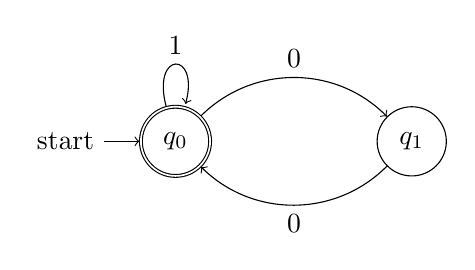
\begin{tikzpicture}[node distance=3cm, on grid, auto] 
   \node[state, initial, accepting] (q0)   {$q_0$}; 
   \node[state] (q1) [right=of q0] {$q_1$}; 
   
   \path[->] 
    (q0) edge [bend left=45] node [above] {0} (q1)
          edge [loop above] node {1} ()
	(q1) edge [bend right=-45] node [below] {0} (q0);
\end{tikzpicture}
\end{center}

Note that there does not exist unique DFAs for a regular language. For the above example, another valid DFA is the following:
\begin{center}
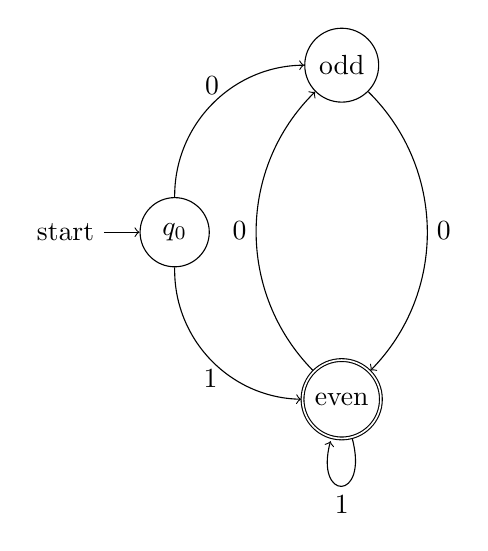
\begin{tikzpicture}[node distance=3cm, on grid, auto] 
   \node[state, initial] (q0)   {$q_0$}; 
   \node[state] (odd) [above right=of q0] {odd}; 
   \node[state, accepting] (even) [below right=of q0] {even}; 
   
   \path[->] 
    (q0) edge [bend left=45] node [above] {0} (odd)
	(q0) edge [bend left=-45] node [below] {1} (even)
	(odd) edge [bend left=45] node [right] {0} (even)
	(even) edge [bend left=45] node [left] {0} (odd)
			edge [loop below] node [below] {1} ();
\end{tikzpicture}
\end{center}

Lets take a look at the algorithm that decides whether a DFA recognizes a string or not:
\begin{lstlisting}
def recognize(dfa: DFA, str: List[Char]): Boolean = {
	var stuck: Boolean = false
	var state = dfa.qo
	
	for (c <- str){
		if (!dfa.transition.definedAt(state, c)){
			stuck = true
		} else {
			state = dfa.transition(state, c)
		}		
	}
	
	!stuck && dfa.accepting.contains(state)
}
\end{lstlisting}

\subsubsection{Intersection of two DFAs}
Suppose you have two DFAs, DFA1 and DFA2. We want a new DFA that accepts a string if and only if its accepted by DFA1 \emph{and} DFA2.\\

Let \(Q_1, Q_2\) be the states of DFA1, DFA2, respectively.\\

Then DFA1 \(\cap\) DFA2 is \((\sum, Q, q_0, A, \delta)\) where:
\begin{itemize}
\item \(Q = Q_1 \times Q_2\) (i.e. the set of all pairs of states of DFA1 and DFA2)
\item \(q_0 = (q_1, q_2)\) (where \(q_1, q_2\) are the starting states of DFA1 and DFA2)
\item \(A = A_1 \times A_2\) (i.e. the set of all pairs of accepting states of DFA1 and DFA2)
\item \(\delta((q_1, q_2), a) = (q_1', q_2')\) if and only if \(\delta(q_1, a) = q_1', \delta(q_2, a) = q_2'\) (i.e. transition to a new state iff the corresponding DFA1 and DFA2 states transition to their new states in DFA1, DFA2 respectively)
\end{itemize}

E.g. Find the intersection of the following two DFAs:
\begin{center}
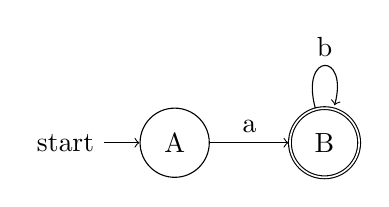
\begin{tikzpicture}
	\node[state, initial] (A) {A};
	\node[state, accepting] (B) [right=of A] {B};
	

	\path[->] 
		(B) edge [loop above] node {b} (B)
	    (A) edge [] node [above] {a} (B);
\end{tikzpicture}
\end{center}

\begin{center}
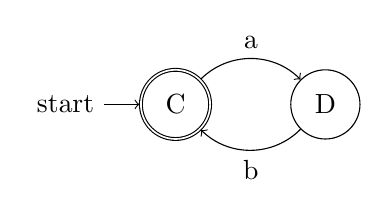
\begin{tikzpicture}
	\node[state, initial, accepting] (C) {C};
	\node[state] (D) [right=of C] {D};
	
	\path[->] 
	    (C) edge [bend left=45] node [above] {a} (D)
	    (D) edge [bend right=-45] node [below] {b} (C);
\end{tikzpicture}
\end{center}

Then the intersection of the two DFAs is:
\begin{center}
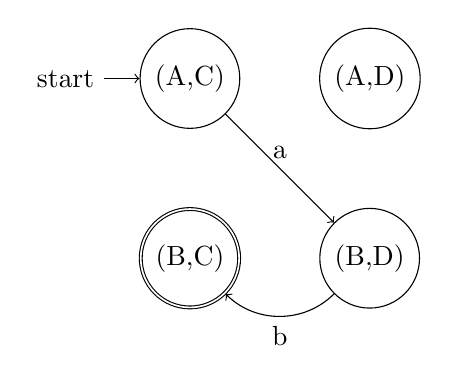
\begin{tikzpicture}
	\node[state, initial] (AC) {(A,C)};
	\node[state] (AD) [right=of AC] {(A,D)};
	\node[state, accepting] (BC) [below=of AC] {(B,C)};
	\node[state] (BD) [right=of BC] {(B,D)};
	
	\path[->] 
	    (AC) edge [] node [above] {a} (BD)
	    (BD) edge [bend right=-45] node [below] {b} (BC);
\end{tikzpicture}
\end{center}


\subsubsection{Non-deterministic Finite Automaton (NFA)}
NFAs are finite state machines that are non-deterministic. This means there can be multiple transitions out of a state on the same symbol.\\

E.g. A sample NFA:

\begin{center}
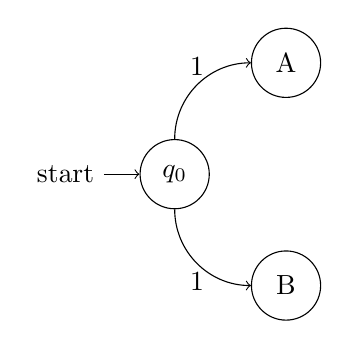
\begin{tikzpicture}[node distance=2cm, on grid, auto] 
   \node[state, initial] (q0)   {$q_0$}; 
   \node[state] (A) [above right=of q0] {A}; 
   \node[state] (B) [below right=of q0] {B}; 
   
   \path[->] 
    (q0) edge [bend left=45] node [above] {1} (A)
	(q0) edge [bend left=-45] node [below] {1} (B);
\end{tikzpicture}
\end{center}

Like DFAs, NFAs are built for a regular language to answer the question whether a string is inside the language.\\

The recognition algorithm for NFAs is slightly different from DFAs as there can now be multiple transitions out of a state on the same symbol. Consider the above example. There are multiple transitions out of \(q_0\) on the symbol 1. We don't know whether following A or B will lead to an accepting state. So the recognition algorithm follows both and checks if at least one of set of resulting end states is an accepting state.\\

A NFA is a 5-tuple \((\sum, Q, q_0, A, \delta)\) where the transition function maps all states and symbols to a set of states you can transition to, \(\delta: Q \times \sum \rightarrow \{S_0, S_1, ..\}\).\\

Lets take a look at the algorithm that decides whether a NFA recognizes a string or not:
\begin{lstlisting}
def recognize(nfa: NFA, str: List[Char]): Boolean = {
	var stuck: Boolean = false

	def recur(state: State, str: List[Char]): List[State] = {
		if (str.isEmpty()){
			List(state)
		} else {
			if (!nfa.transition	.definedAt(state, str.head)){
				stuck = true
			} else {
				nfa.transition(state, str.head).flatMap(
					(newState: State) => recur(newState, str.tail))
			}
		}
	}

	!stuck && recur(nfa.qo, str).exists(nfa.accepting.contains)
}
\end{lstlisting}

\subsubsection{Epsilon-NFAs}
An \(\epsilon\)-NFA is a NFA that has epsilon transitions. An epsilon transition is a transition to another state without consuming a symbol.\\

E.g. A sample \(\epsilon\)-NFA

\begin{center}
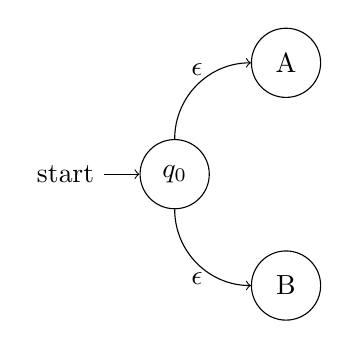
\begin{tikzpicture}[node distance=2cm, on grid, auto] 
   \node[state, initial] (q0)   {$q_0$}; 
   \node[state] (A) [above right=of q0] {A}; 
   \node[state] (B) [below right=of q0] {B}; 
   
   \path[->] 
    (q0) edge [bend left=45] node [above] {$\epsilon$} (A)
	(q0) edge [bend left=-45] node [below] {$\epsilon$} (B);
\end{tikzpicture}
\end{center}

\subsubsection{Regular Expressions}
Regular expressions are an alternate way of specifying a regular language compared to building a DFA, NFA, or \(\epsilon\)-NFA for it.\\

Like DFAs, NFAs and \(\epsilon\)-NFA, regular expressions are built for a regular language to answer the question whether a string is inside the language.\\

A regular expression is defined as the following:
\begin{enumerate}
\item \(R := \epsilon\). A regular expression can be the empty string. The language this regular expression specifies is L = \(\{\epsilon\}\). It only accepts the empty string.
\item \(R := a, a \in \sum\). A regular expression can be a symbol from the alphabet. The language this regular expression specifies is \(L = \{a\}\). It only accepts the symbol a.
\item \(R := R_1|R_2\). A regular expression can be the OR of two regular expressions. The languages specified is \(L = L_1 \cup L_2\). It will accept any string that is either in \(L_1\) or \(L_2\), or both.
\item \(R := R_1 R_2\). A regular expression can be the concatenation of two regular expressions. The language specified is \(L = \{uv | u \in L_1, v \in L_2\}\). It accepts any string such that the first part of the string is inside \(L_1\) and the second part is inside \(L_2\).
\item \(R := R_1^*\). A regular expression can be 0 or more concatenations of a regular expression. The language specified is \(L = \{\epsilon\} \cup L_1 \cup L_1L_1 \cup L_1L_1L_1 \cup ...\). It will accept any string that is the result of 0 or more concatenations of strings that are inside \(L_1\).
\end{enumerate}

E.g. \(R = \epsilon\). \(L = \{\epsilon\}\).\\

E.g. \(\sum = \{a, b, c, ..., z\}\). \(R = a\). \(L = \{a\}\).\\

E.g. \(R = a|b\). \(L_1 = \{a\}\), \(L_2 = \{b\}\), \(L = \{a, b\}\).\\

E.g. \(R = (a|b)|c\). \(L_1 = \{a, b\}\), \(L_2 = \{c\}\), \(L = \{a, b, c\}\).\\

E.g. \(R = ab\). \(L_1 = \{a\}\), \(L_2 = \{b\}\), \(L = \{ab\}\).\\

E.g. \(R = abc\). \(L_1 = \{ab\}\), \(L_2 = \{c\}\), \(L = \{abc\}\).\\

E.g. \(R = (ab)^*\). \(L_1 = \{ab\}\), \(L = \{\epsilon, ab, abab, ababab, abababab, ...\}\).\\

E.g. \(R = a(a)^*\). \(L = \{a, aa, aaa, aaaa, ...\}\).\\

Kleenes Theorm: Given a regular language L there exists a DFA specifying L, NFA specifying L, \(\epsilon\)-NFA specifying L and a regular expression specifying L.\\

E.g. Give a regular expression for a language of all english words containing the word "issi":

\(R = (A-z)^*(issi)(A-z)^*\)\\

E.g. Give a regular expression for a language of all binary strings with even block of 0's and even block of 1's:

\(R = ((00)^*(11)^*)^*\)

\subsubsection{Scanning}
Scanning deals with the problem of tokenization. That is, given a regular language L and a string, break the string down into a set of tokens that are in the language.\\

E.g. Suppose L = C++ and we have the string "int main()\{ return 0; \}".

We want to convert this string to a set of tokens that are in the C++ language. \{int, main, (, ), \{, return, 0, ;, \}\}.\\

We will study one algorithm that makes uses of DFAs to solve the problem of tokenization, called Maximal munch.\\

The basic idea of maximal munch is to use as much of the string to generate tokens.\\

E.g. Let L = \(\{aa, aaa\}\) and w = "aaaaa". Maximal munch will use as much of the string as possible to generates tokens and return \(\{aaa, aa\}\). Note that the tokenization \(\{aa, aaa\}\) is still valid.\\

In general, scanning output is not unique. There can be many valid of tokenizations of a string. Maximal munch chooses the longest possible token for each tokenization step as a way to ensure unique output.\\

E.g. Let L = \(\{aa, aaa\}\) and w = "aaaa". Maximal munch will produce the first largest token as "aaa", then attempt to tokenize "a". However there exists no valid tokenization of "a". So maximal munch will produce an error. Note that there exists a valid tokenization of the string, \(\{aa, aa\}\).\\

In general, maximal munch will not always find a valid tokenization, even if it exists.\\

Lets take a look at the algorithm. Given: a regular language L, a DFA of that language, a string w:
\begin{enumerate}
\item Run the DFA on w.
\item If the resulting end state is an accepting state, return w as a token.
\item If not, go back to the last accepting state.
\item If there is no last accepting state then return an error.
\item Otherwise, generate the token of the last accepting state and rerun this algorithm on the rest of the string.
\end{enumerate}

\newpage

\section{Context Free Languages and Parsing}
Suppose we now want to scan expressions. We could try doing this using DFAs. \\

E.g. Lets write a DFA to recognize the expression \(a + b * c - d\):
\begin{center}
\begin{tikzpicture}
	\node[state, initial] (q0) {$q_0$};
	\node[state, accepting] (exp) [right=of C] {Exp};
	
	\path[->] 
	    (q0) edge [bend left=45] node [above] {ID} (exp)
	    (exp) edge [bend right=-45] node [below] {+, -, *, /} (q0);
\end{tikzpicture}
\end{center}

E.g. Now suppose we add brackets to the expression: \((a + b) * (c - d)\). The above DFA does not recognize this expression even though it is valid. Lets instead write a new DFA:
\begin{center}
\begin{tikzpicture}[node distance=2cm]
	\node[state, initial] (q0) {$q_0$};
	\node[state, accepting] (exp) [right=of C] {Exp};
	\node[state] (left) [below=of q0] {};
	\node[state] (right) [right=of left] {};	
	
	\path[->] 
	    (q0) edge [bend left=45] node [above] {ID} (exp)
	    (q0) edge [bend right=45] node [left] {(} (left)
	    (exp) edge [bend right=-45] node [below] {+, -, *, /} (q0)
   	    (left) edge [bend left=45] node [above] {ID} (right)
	 	(right) edge [bend right=45] node [right] {)} (exp)
	    (right) edge [bend right=-45] node [below] {+, -, *, /} (left);
\end{tikzpicture}
\end{center}

But now this DFA doesn't work for the expression \((a + b) * ((c) - d)\). We would need to add another state to accept double open brackets. But even that DFA would not work for an expression with 3 open brackets.\\

In general, regular languages and ways of specifying regular languages are not sufficient for nested structures like expressions and procedures. The reason why is because DFAs, NFAs, \(\epsilon\)-NFAs all depend on knowing the number of previous symbols that it encountered. For example, we could be in a state called "(((" which means we've encountered 3 open brackets. Similarly, there would be states "((((", "(((((". Each state tells us something about the previous symbols that it encountered.\\

Now consider a nested structure like expressions which can have an arbitrary number of open and close brackets. To write a DFA/NFA/\(\epsilon\)-NFA for this structure we would need an arbitrary number of states, which is not possible. We need another concept to represent nested structures, like context free languages.\\

The main idea of context free languages is to replace looping by recursion. As a result, many context free definitions are recursive definitions.\\

Context free grammar is a 4-tuple \((V, \sum, P, s)\) where:
\begin{itemize}
\item V is a finite set of non-terminals
\item \(\sum\) is a finite set of terminals (also known as the alphabet)
\item P is a finite set of production rules (also known as grammar rules)
\item s is the starting non-terminal
\end{itemize}

A non-terminal symbol expands to something else. That is, it does not terminate. A terminal symbol does not expand to something else. That is, it terminates.\\

E.g. Consider the following context free grammar production rules for an expression:\\

exp \(\rightarrow\) ID \(\vert\) exp op exp\\
op \(\rightarrow\) + \(\vert\) - \(\vert\) * \(\vert\) /\\

In this grammar the terminals are \(\sum = \) \{ID, +, -, *, /\} because they do not expand to anything else in the production rules. The non-terminals are V = \{exp, op\} because they expand to something else in the production rules\footnote{Note that anything to the left-hand side of the production rules are non-terminals.}. By convention, the starting non-terminal is the first non-terminal, exp.\\

We can use this grammar to generate a parse tree of an expression.\\

E.g. Parse tree of a + b * c:
\begin{center}
\Tree [.exp [.exp [.exp [.ID a ] ] [.op + ] [.exp [.ID b ] ] ] 
			[.op * ] 
			[.exp [.ID c ] ] ]
\end{center}

Conventions with context free grammar:
\begin{itemize}
\item a, b, c, d, \(\in \sum\) (i.e. The symbols a, b, c, d refer to a terminal)
\item A, B, C, D, S \(\in V\). (i.e. The symbols A, B, C, D, S refer to a non-terminal)
\item W, X, Y, Z \(\in (\sum \cup V)\). (i.e. The symbols W, X, Y, Z refer to a terminal or non-terminal)
\item w, x, y, z \(\in \sum^*\). (i.e. The symbols w, x, y, z refer to sequences of terminals)
\item \(\alpha, \beta, \gamma \in (\sum \cup V)^*\). (i.e. The symbols \(\alpha, \beta, \gamma\) refer to sequences of terminals and non-terminals)
\end{itemize}

We say:\\

\(\alpha\) A \(\beta \underbrace{\Rightarrow}_\text{directly derives} \alpha\) \(\gamma\) \(\beta\) if \(\{A \rightarrow \gamma\} \in P\).\\

\(\alpha_1 \underbrace{\Rightarrow^*}_\text{derives} \alpha_n\) if there is a chain of directly derives leading from \(\alpha_1\) to \(\alpha_n\) (i.e. \(\alpha_1 \Rightarrow \alpha_2 \Rightarrow ... \Rightarrow \alpha_n\)).\\

E.g. exp \(\Rightarrow\) exp op exp\\

E.g. exp \(\Rightarrow^*\) ID + ID since exp \(\Rightarrow\) exp op exp \(\Rightarrow\) exp + exp \(\Rightarrow\) ID + exp \(\Rightarrow\) ID + ED\\

The language generated by a context free grammar G = \((V, \sum, P, s)\) is L = \(\{w \in \sum^* \vert s \Rightarrow^* w\}\). That is, the language generated by G is a set of sequences of terminals that the starting non-terminal derives.\\

We say a context free grammar is ambiguous if there exists multiple valid parse trees for an expression. Otherwise it is unambiguous. \\

E.g. The context free grammar introduced in the last example is ambiguous. Consider the two valid parse trees for the expression a + b * c.\\

\begin{minipage}[t]{0.5\textwidth}
\begin{center}
\Tree [.exp [.exp [.exp [.ID a ] ] [.op + ] [.exp [.ID b ] ] ] 
			[.op * ] 
			[.exp [.ID c ] ] ]
\end{center}
\end{minipage}
\begin{minipage}[t]{0.5\textwidth}
\begin{center}
\Tree [.exp [.exp [.ID a ] ]
			[.op + ] 
			[.exp [.exp [.ID b ] ] [.op * ] [.exp [.ID c ] ] ] ]
\end{center}
\end{minipage}

\vspace{7mm}

In the above example, which parse tree is correct? Bedmas tells us its the one on the right but there are expressions where even applying bedmas can result in multiple valid parse trees, such as a - b - c.\\

In general, we want to specify languages precisely and get a unique parse (just like we want a unique scan). That is, we want to work with unambiguous grammar. However, the problem of figuring out whether a grammar is unambiguous is a undecidable by an algorithm. As a result, we often have to come up with a grammar and make sure it is unambiguous through rigorous testing. Fortunately, the grammar for the language we are implementing on the assignments, Lacs, is unambiguous.\\

E.g. Example of a unambiguous context free grammar. There exists only one valid parse tree for the expression a - b - c:\\

exp \(\rightarrow\) term \(\vert\) exp + term \(\vert\) exp - term\\
term \(\rightarrow\) ID \(\vert\) term * ID \(\vert\) term / ID\\

\begin{center}
\Tree [.exp [.exp [.exp [.term [.ID a ] ] ] [-  ] [.term [.ID b ] ] ]
			[-  ]
			[.term [.ID c ] ] ]
\end{center}

\subsubsection{Parsing}
Parsing deals with the problem of generating a parse tree for a sequence of terminals. The sequence of terminals are the sequence of tokens we got from running the scanner on our input program.\\

We will study one algorithm for generating a parse tree, called the CYK algorithm.\\

The first question we need to answer is whether \(\alpha \Rightarrow^* x\). After we implement the algorithm to answer that question, we will extend it to generate a parse tree if \(\alpha \Rightarrow^* x\) is true.\\

There are 4 sub cases to handle:
\begin{enumerate}
\item \(\alpha = \epsilon\). When does \(\epsilon \Rightarrow^* x\)? The only time \(\epsilon\Rightarrow^* x\) is when \(x = \epsilon\).
\item \(\alpha = a\beta\). Note that \(a\) is a terminal symbol. That means anything \(\alpha\) derives has to start with \(a\) since \(a\) cannot expand to anything else. When does \(a\beta \Rightarrow^* x\)? The only time this happens is when \(x = az\) and \(\beta \Rightarrow^* z\).
\item \(\alpha = A\). In this case we need to expand \(A\) and go through all of its production rules. That is, for all \(\gamma\), \(A \rightarrow \gamma \in P\), we need to check if \(\gamma \Rightarrow^* x\). If at least one \(\gamma \Rightarrow^* x\) then \(A \Rightarrow^* x\). If not, then \(A \nRightarrow^* x\).
\item \(\alpha = A\beta\). When does \(A\beta \Rightarrow^* x\)? We need to split \(x\) into all possible sub-strings, \(x_1, x_2\), and check if \(A \Rightarrow^* x_1\) and \(\beta \Rightarrow^* x_2\). If at least one of these is true for some sub-string \(x_1, x_2\), then \(A\beta \Rightarrow^* x\).
\end{enumerate}

\begin{lstlisting}[escapeinside={(*}{*)}]
def parse((*$\alpha, x$*)) = {
	if ((*$\alpha$*).isEmpty()){
		return (*$x$*).isEmpty()
	} else if ((*$\alpha = a\beta$*)){
		return (*$x = az$*) && parse((*$\beta, z$*))
	} else if ((*$\alpha = A$*)){
		for each production rule: (*$A \rightarrow \gamma \in P$*) {
			if (parse((*$\gamma, x$*)){
				return true
			}
		}
		
		return false
	} else {
		(*$\alpha = A\beta$*)
		for each ((*$x = x_1x_2$*)) {
			if (parse((*$A, x_1$*)) && parse((*$\beta, x_2$*)){
				return true
			}
		}
		
		return false
	}
}
\end{lstlisting}

Lets run the algorithm on an example to see if there are any bugs.\\

E.g. Run the CYK parsing algorithm on parse(\(exp \Rightarrow^* ID + ID\)).

Recall the context free grammar:\\

exp \(\rightarrow\) ID \(\vert\) exp op exp\\
op \(\rightarrow\) + \(\vert\) - \(\vert\) * \(\vert\) /

\begin{itemize}
	\item [3.] Notice that \(exp = A\). For each production rule:
	\begin{itemize}
		\item [-] parse(\(ID \Rightarrow^* ID + ID\))? Notice that \(ID = a\beta\) where \(a = ID, 			\beta = \epsilon\).
		\begin{itemize}
			\item [2.] We see that \(x = az\) where \(a = ID, z =\) + \(ID\). Does parse(\(\epsilon 			\Rightarrow^* + \) \(ID\))?
			\begin{itemize}
				\item [1.] We see that \(+\) \(ID \neq \epsilon\), return false.
			\end{itemize}
		So parse(\(ID \Rightarrow^* ID + ID\)) is false.
		\end{itemize}
		\item [-] parse(\(exp\) \(op\) \(exp \Rightarrow^*\) \(ID\) + \(ID\))? Notice that \(exp\) \(op\) \(exp\) = \(A\beta\) where \(A = exp, \beta =\) \(op\) \(exp\).
			\begin{itemize}
				\item [4.] What are all the different ways to split \(ID\) + \(ID\)? \(\{(\epsilon, ID + ID), (ID, +\) \(ID), (ID\) \(+, ID), (ID + ID, \epsilon)\}\). 
				\begin{itemize}
					\item [-] parse(\(exp\) \(\Rightarrow^* \epsilon\)) and parse(\(op\) \(exp\) \(\Rightarrow^* ID + ID\)). Lets first focus on parse(exp \(\Rightarrow^* \epsilon\)). Notice that \(exp = A\). parse(\(ID \Rightarrow^* \epsilon\))? False. parse(\(exp\) \(op\) \(exp\) \(\Rightarrow^* \epsilon\))? This leads to answering the question parse(\(exp \Rightarrow^* \epsilon\)) which is an infinite loop.
					\item [-] parse(\(exp \Rightarrow^* ID\)) and parse(\(op\) \(exp\) \(\Rightarrow^*\) \(+\) \(ID\)). Lets focus on parse(\(exp \Rightarrow^* ID\)). True. And so on...
				\end{itemize}
			\end{itemize}
	\end{itemize}
\end{itemize}

We see that the algorithm runs fine on the example except there is an infinite loop. We wanted to figure out whether parse(\(exp \Rightarrow^* \epsilon\)) but, as a process of figuring that out, we asked whether parse(\(exp \Rightarrow^* \epsilon\)). This is an infinite loop.\\

In order to fix this we can apply memoization to the algorithm. The basic idea of memoization is: if you have to compute the result twice, just use the previous result. Whenever we need to compute \(\alpha \Rightarrow^* x\), check the memo table. If we've computed it before, return the result from the memo table. Otherwise, compute \(\alpha \Rightarrow^* x\) and update the memo table.\\

Furthermore, we can use memoization to fix the infinite loop in the algorithm. Before the start of the core algorithm of checking whether \(\alpha \Rightarrow^* x\), set the value in the memo table to be false. So now, if the algorithm attempts to answer the question \(\alpha \Rightarrow^* x\) again, it will check the memo table and return false.\\

What is the space complexity of the parsing CYK algorithm? We can figure this out by looking at the memo table.

\begin{lstlisting}[escapeinside={(*}{*)}]
val memo = Map[((*$\underbrace{Seq[Symbol]}_\text{$\alpha$}$*), (*$\underbrace{Int}_\text{from}$*), (*$\underbrace{Int}_\text{length}$*)), Option[Seq[Tree]]]
\end{lstlisting}

What are all the possible values for \(\alpha\)? 

We know \(\alpha\) starts as the starting non-terminal and, after that, is always a prefix or suffix of some right hand side production rule. Since our context free grammar has finite production rules, there are finite many possible values for \(\alpha\). From and length are used to refer to a substring of \(x\) in an efficient way and there are \(O(\vert x \vert)\) many possibilities for each of them. So the space time complexity is \(O(\vert 1 \vert) * O(\vert x \vert) * O(\vert x \vert) = O(\vert x^2 \vert)\).\\

What is the running time complexity of the parsing CYK algorithm? 

At worst, the entire memo table is filled. So it is \(\Omega(x^2)\). We also need to account for the time it takes to split a string into all possible sub strings, \(O(\vert x \vert)\). So the run time complexity is \(O(\vert x^3 \vert)\).\\

How can we modify the algorithm to generate a parse tree if \(\alpha \Rightarrow^* x\)? Lets consider all 4 sub cases:

\begin{enumerate}
\item parse(\(\epsilon \Rightarrow^* \epsilon\)). Return empty sequence of tree nodes.
\item parse(\(a\beta \Rightarrow^* az\)). Return Tree(a, []) +: parse(\(\beta \Rightarrow^* z\)).
\item parse(\(A \Rightarrow^* x\)) and there exists \(\gamma\), \(A \rightarrow \gamma \in P\), such that parse(\(\gamma \Rightarrow^* x\)). Return Tree(\(A\), parse(\(\gamma \Rightarrow^* x\))).
\item parse(\(A\beta \Rightarrow^* x\)) and there exists \(x = x_1x_2\) such that parse(\(A \Rightarrow^* x_1\)) and parse(\(\beta \Rightarrow^* x_2\)). Return parse(\(A \Rightarrow^* x_1\)) ++ parse(\(\beta \Rightarrow^* x_2\)).
\end{enumerate}

\subsubsection{Parsing Algorithms Comparison}
\begin{itemize}
\item [] Parsing CYK. Advantages: General, easy to learn, works for all grammars. Disadvantages: Space complexity is large, \(O(\vert x^2 \vert)\) and time complexity is large, \(O(\vert x^3 \vert)\).
\item [] LR(1)/LR(k). Advantages: Efficient, \(O(\vert x \vert)\). Can use LR(1) parsers to test for ambiguity (if it can be parsed by LR(1) then grammar is unambiguous). Disadvantages: Takes 3 weeks to learn. Works for most unambiguous practical grammars but not all.
\item [] LL(1)/LL(k). Advantages: Efficient, \(O(\vert x \vert)\). Disadvantages: Takes 1.5 weeks to learn. Works for few grammars. Always generates a right associative parse tree.
\item [] Earley parser. Advantages: Works for all grammars. Moderately efficient. Running time is \(O(\vert x^2 \vert)\) on unambiguous grammar and \(O(\vert x^3 \vert)\) on ambiguous grammar. Disadvantages: LR(1)/LR(k) parsers can parse most grammars in \(O(\vert x \vert)\).
\end{itemize}

\subsubsection{Correct Prefix Property}
Suppose that you have a program that you spent a long time building and try compiling it. However, there is a syntax error in the program and so the parsing CYK algorithm cannot generate a parse tree for the program. It would be nice to know why the parse tree cannot be generated to help debug the syntax error.\\

A parser has the correct prefix property if it halts as soon as it encounters a terminal symbol that cannot possibly make a parse tree.\\

Suppose \(w\) is a sequence of terminals that represents a program. Let \(w = xaz\) where \(w \not\in Language\). Then \(w\) does not have a parse tree.\\

Suppose that \(\exists y, xy \in Language\). That is, its possible for some part of \(w\) to be in the language and have a parse tree. Then we know \(\forall v, xav \not\in Language\).\\

A parser has the correct prefix property if it rejects the program as soon as it encounters \(a\) (a terminal that cannot make a parse tree). Most parsers have this property except the parsing CYK algorithm.

\newpage

\section{Context Sensitive Analysis}
Context sensitive analysis deals with rejecting incorrect programs, resolving names and performing type checking.

\subsubsection{Rejecting incorrect programs}
We need to reject programs that have duplicate names and undeclared names. We will do this during type checking.

\subsubsection{Resolving names}
Every ID token in Lacs is used to refer to a variable or a procedure. We need to map all names to either a variable or a procedure.\\

E.g. Consider the following code:
\begin{lstlisting}
def f(): Int = {
	var y: Int = 10;
	
	def p(): Int = {
		var x: Int = 5;
		x + y
	}
	
	def q(): Int = {
		var x: Int = 6;
		x + y	
	}
	
	y
}
\end{lstlisting}
The procedures p() and q() both have a variable \(x\). This is valid because a variable can mean different things depending on its scope. Also notice that p() and q() can access \(y\), a variable declared in f()'s scope.\\

In general, to resolve names, we need to build a symbol table that maps names to variables or procedures, for \emph{every} procedure scope. Furthermore, any procedure that is nested within another procedure should inherit the parent procedure's symbol table.\\

E.g. Consider the following code:
\begin{lstlisting}
def f(): Int = {
	var x: Int;
	
	def g(): Int = {
		var x: Int;
		x = 5;
		x
	}
	
	x =  6;
	x
}
\end{lstlisting}
Notice that inside g()'s scope \(x\) means 5 not 6.\\

In general, nested procedures need to inherit and shadow their parent procedure's symbol table. Any outer variable that is declared with the same name as an inner variable needs to be overwritten by the inner procedure.

\subsubsection{Type checking}
In Lacs there are two types:
\begin{itemize}
\item 2's complement integers between \(-2^{31}\) to \(2^{31} - 1\) with arithmetic module \(2^{32}\)
\item Function values that represent a function that takes arguments with specified types and returns a return type (E.g. \((Int, Int) \Rightarrow Int\))
\end{itemize}

A type system is a set of rules that computes the type of an expression based on the types of its sub-expressions. We can follow these rules to determine the type of any expression.\\

A type system is sound if whenever the type system computes a type \(\tau\) for an expression, the expression actually evaluates to a value of type \(\tau\). Essentially it means the type system is not lying. Fortunately, the Lacs type system is sound.

\subsubsection{Lacs Type System}
Let \(E \in\) \{expras, expra, expr, term, factor\} and \(\tau \in\) \{type\}. Note that \(\Gamma \vdash E:\) \textbf{Int} means if we type check \(E\), we get an Int. \(\Gamma(E)\) means getting the expression's type from the symbol table. Everything above the overbar are conditions for the rule to be true.\\

\begin{enumerate}
\item Literals\\

$\overline{\Gamma \vdash \textbf{NUM}: \textbf{Int}}$

\item IDs\\

$\overset{\displaystyle \Gamma(\textbf{ID}) = \tau}{\overline{\Gamma \vdash \textbf{ID}: \tau}}$

\item Parenthesis\\

$\overset{\displaystyle \Gamma \vdash E: \tau}{\overline{\Gamma \vdash (E): \tau}}$

\item Arithmetic\\

$\overset{\displaystyle \Gamma \vdash E_1: \textbf{Int}, \ \Gamma \vdash E_2: \textbf{Int}}{\overline{\Gamma \vdash E_1 \ \{+, -, *, /\} \ E_2: \textbf{Int}}}$

\item Assignment\\

$\overset{\underline{\displaystyle \Gamma(\textbf{ID}) = \tau, \ \Gamma \vdash E: \tau}}{\Gamma \vdash \textbf{ID} = E: \tau}$

\item Sequence of expression\\

$\overset{\underline{\displaystyle \Gamma \vdash E_1: \tau', \ \Gamma \vdash E_2: \tau}}{\Gamma \vdash E_1; E_2: \tau}$

Note that we still need to type check \(E_1\) to make sure its valid and has a type. Otherwise, \(E_1\) could be an invalid expression.

\item If statements\\

$\overset{\displaystyle \Gamma \vdash E_1: \textbf{Int}, \ \Gamma \vdash E_2: \textbf{Int}, \ \Gamma \vdash E_3: \tau, \ \Gamma \vdash E_4: \tau}{\overline{\Gamma \vdash \textbf{if} \ (E_1 \ \{==, !=, >=, <=, >, <\} \ E_2)\ E_3 \ \textbf{else} \ E_4: \tau}}$

In an if statement, the thens and elses block must return a value of the same type.

\item Procedure call\\

$\overset{\underline{\displaystyle \Gamma \vdash E'(\overline{\tau}) \Rightarrow \tau', \ \forall i. \ \Gamma \vdash E_i: \tau_i}}{\Gamma \vdash E'(\overline{E}): \tau'}$

The parameter and argument types must match.

\item Procedure Declaration\\

$\overset{\underline{\displaystyle \Gamma + \overline{\text{vardef}} + \overline{\text{vardef'}} + \overline{\text{defedef}} \vdash \forall i. \text{defdef}_i, \ \Gamma + \overline{\text{vardef}} + \overline{\text{vardef'}} + \overline{\text{defedef}} \vdash E: \tau}}{\Gamma \vdash \textbf{def ID}(\overline{\text{vardef}}): \tau = \{\overline{\text{vardef'}}, \overline{\text{defdef}}, E\}}$

As mentioned before, we need to make sure there are no duplicate names. So all names in \(\overline{\text{vardef}}\), \(\overline{\text{vardef'}}\), \(\overline{\text{defdef}}\) need to be distinct, that is, all parameter names, variable names and nested procedure names need to be distinct.\\

We need to type check each of the procedure's nested procedures. However, recall that every nested procedure should inherit and shadow their parent procedure's symbol table. Therefore we need to update the symbol table with the newly added parameters, variables and nested procedures names before we type check each nested procedure.\\

We also need to type check \(E\) to make sure it is the same as the procedure's return type.

\item Program\\

$\overset{\underline{\displaystyle \emptyset + \ \overline{\text{defdef}} \vdash \forall i. \ \text{defdef}_i}}{\emptyset \vdash \overline{\text{defdef}}}$

In Lacs a program is just a sequence of top level procedures. In order to type check a program we need to type check all top level procedures. However, recall that top level procedures can call each other. Therefore we need to update the empty symbol table with all the top level procedures names.
\end{enumerate}

\newpage

\section{Memory Management}
A heap is a data structure that manages memory so that it can be allocated and freed at any time.\\

There are two key functions of a heap:
\begin{itemize}
\item Allocate a new chunk of a given size
\item Deallocate a  chunk, returning it back into the memory pool so it can be used later
\end{itemize}

Deallocation can be explicit (like in C/C++) or explicit (like in Java, Scala). We will study both of these topics, starting with how to implement an early day C heap.

\subsubsection{Early day C Memory Management}
Main idea: use a linked list of free chunks. This linked list will contain all chunks that are currently free in the heap.\\

Every chunk needs to store a next pointer that points to the next free chunk in the linked list.

\[
\begin{tabular}{|c|}
\hline
size of chunk\\
\hline
next pointer\\
\hline
data\\
..\\
\hline
\end{tabular}
\]\\

Convention: The heapStart register will store the head of the linked list. A chunk's next pointer will point to one word after the end of the heap to indicate that it is the last chunk in the linked list.\\

Suppose we want to allocate a chunk of a given size but the only large enough free chunk is the head of the linked list. Then we would need to update the head of the linked list. In order to avoid this case, we will use a dummy head.\\

The initialization code for the heap will need to initialize the dummy head and set the next pointer to a chunk that is almost the size of the entire heap.\\

\begin{lstlisting}
def setSize(chunk, size) = assignToAddr(chunk, size)

def setNext(chunk, next) = assignToAddr(chunk + 4, next)

def init() = {
	setSize(heapStart, 8)
	val newChunk = heapStart + 8
	setSize(newChunk, heapSize - 8)
	setNext(heapStart, newChunk)
	setNext(newChunk, heapStart + heapSize)
}
\end{lstlisting}
So now the linked list looks as follows:
\begin{center}
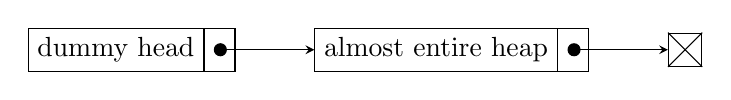
\begin{tikzpicture}[list/.style={rectangle split, rectangle split parts=2,
    draw, rectangle split horizontal}, >=stealth, start chain]

  \node[list,on chain] (A) {dummy head};
  \node[list,on chain] (B) {almost entire heap};
  \node[on chain,draw,inner sep=6pt] (D) {};
  \draw (D.north east) -- (D.south west);
  \draw (D.north west) -- (D.south east);
  \draw[*->] let \p1 = (A.two), \p2 = (A.center) in (\x1,\y2) -- (B);
  \draw[*->] let \p1 = (B.two), \p2 = (B.center) in (\x1,\y2) -- (D);
\end{tikzpicture}
\end{center}

Suppose we want to allocate a chunk of size: wanted. We need to find a chunk inside the linked list of free chunks that has size at least wanted + 8 and then remove it from the linked list (as it is no longer free).\\

In order to remove a node from a linked list we need to set prev.next = curr.next:
\begin{center}
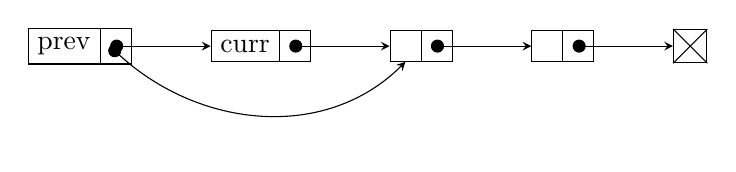
\begin{tikzpicture}[list/.style={rectangle split, rectangle split parts=2,
    draw, rectangle split horizontal}, >=stealth, start chain]

  \node[list,on chain] (A) {prev};
  \node[list,on chain] (B) {curr};
  \node[list,on chain] (C) {};
  \node[list,on chain] (D) {};    
  \node[on chain,draw,inner sep=6pt] (E) {};
  \draw (E.north east) -- (E.south west);
  \draw (E.north west) -- (E.south east);
  \draw[*->] let \p1 = (A.two), \p2 = (A.center) in (\x1,\y2) -- (B);
  \draw[*->] let \p1 = (B.two), \p2 = (B.center) in (\x1,\y2) -- (C);
  \draw[*->] let \p1 = (C.two), \p2 = (C.center) in (\x1,\y2) -- (D);  
  \draw[*->] let \p1 = (D.two), \p2 = (D.center) in (\x1,\y2) -- (E);
  \draw[*->] let \p1 = (A.two), \p2 = (A.center) in (\x1,\y2) to[out=-45,in=-135] (C);      
\end{tikzpicture}
\end{center}

Suppose we find a chunk that is much bigger than wanted + 8. If we just gave that chunk to the user the heap would be full immediately. So we need to detect if a chunk is too big for the size the user wanted and, if so, split it into two chunks: one that has size wanted + 8 and another chunk that is the leftover chunk.\\

\begin{minipage}[t]{0.5\textwidth}
\begin{center}
Large chunk\\
\begin{tabular}{|c|}
\hline
Size \(\geq\) wanted + 8\\
\hline
next\\
\hline
..\\
..\\
\hline
\end{tabular}
\end{center}
\end{minipage}
\begin{minipage}[t]{0.5\textwidth}

\begin{center}
User's chunk\\

\begin{tabular}{|c|}
\hline
Size = wanted + 8\\
\hline
next\\
\hline
..\\
..\\
\hline
\end{tabular}\\

\vspace{7mm}

Leftover chunk\\

\begin{tabular}{|c|}
\hline
Size \(\geq\) 8\\
\hline
next\\
\hline
..\\
..\\
\hline
\end{tabular}
\end{center}
\end{minipage}

\vspace{7mm}

\begin{lstlisting}[escapeinside={(*}{*)}]
def size(chunk) = deref(chunk)

def next(chunk) = deref(chunk + 4)

def malloc(wanted) = {
	def find(prev) = {
		val current = next(prev)
		
		if (size(current) < wanted + 8){
			find(current)
		} else {
			if (size(current) (*$\geq$*) wanted + 16){
				val newChunk = current + (wanted + 8)
				setSize(newChunk, size(current) - (wanted + 8))
				setSize(current, wanted + 8)
				setNext(prev, newChunk)
				setNext(newChunk, next(current))
			} else {
				setNext(prev, next(current))
			}
		}
	}
	
	find(heapStart)
}
\end{lstlisting}
Note that we need to add the leftover chunk into the linked list since it is a free chunk.\\

Suppose the user wants to deallocate a chunk, called toFree. We need to add it back into the linked list since it will be a free chunk after deallocation. Suppose we add toFree back into the linked list and it is directly above or below another chunk that is free. We would want to merge these free chunks together into one, otherwise the user may not be able to allocate a large chunk. There are 4 sub cases to deal with:\\

\begin{enumerate}
\item Chunks before and after toFree are both non-free:

\begin{center}
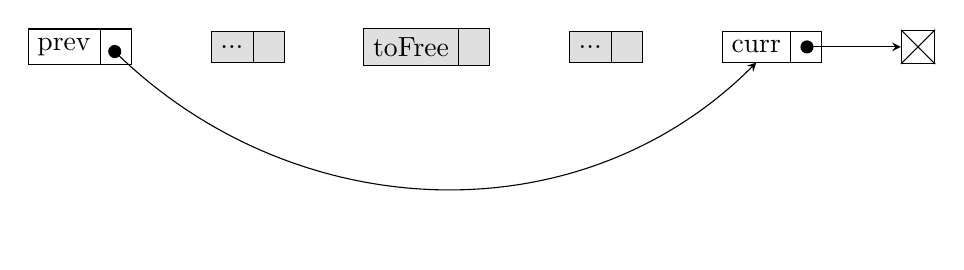
\begin{tikzpicture}[list/.style={rectangle split, rectangle split parts=2,
    draw, rectangle split horizontal}, >=stealth, start chain]

  \node[list,on chain] (A) {prev};
  \node[list,on chain, fill=gray!25] (B) {...};
  \node[list,on chain, fill=gray!25] (C) {toFree};
  \node[list,on chain, fill=gray!25] (D) {...};    
  \node[list,on chain] (E) {curr};
  \node[on chain,draw,inner sep=6pt] (F) {};
  \draw (F.north east) -- (F.south west);
  \draw (F.north west) -- (F.south east);
  \draw[*->] let \p1 = (A.two), \p2 = (A.center) in (\x1,\y2) to[out=-45,in=-135] (E);
  \draw[*->] let \p1 = (E.two), \p2 = (E.center) in (\x1,\y2) -- (F);
\end{tikzpicture}
\end{center}

\begin{center}
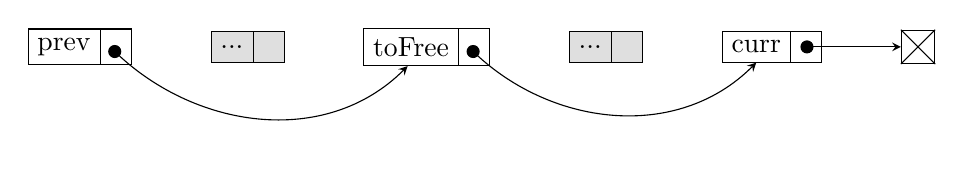
\begin{tikzpicture}[list/.style={rectangle split, rectangle split parts=2,
    draw, rectangle split horizontal}, >=stealth, start chain]

  \node[list,on chain] (A) {prev};
  \node[list,on chain, fill=gray!25] (B) {...};
  \node[list,on chain] (C) {toFree};
  \node[list,on chain, fill=gray!25] (D) {...};    
  \node[list,on chain] (E) {curr};
  \node[on chain,draw,inner sep=6pt] (F) {};
  \draw (F.north east) -- (F.south west);
  \draw (F.north west) -- (F.south east);
  \draw[*->] let \p1 = (A.two), \p2 = (A.center) in (\x1,\y2) to[out=-45,in=-135] (C);
  \draw[*->] let \p1 = (C.two), \p2 = (C.center) in (\x1,\y2) to[out=-45,in=-135] (E);
  \draw[*->] let \p1 = (E.two), \p2 = (E.center) in (\x1,\y2) -- (F);
\end{tikzpicture}
\end{center}

We need to:
\begin{lstlisting}
prev.next = toFree
toFree.next = curr
\end{lstlisting}

\item Chunk after toFree is free:

\begin{center}
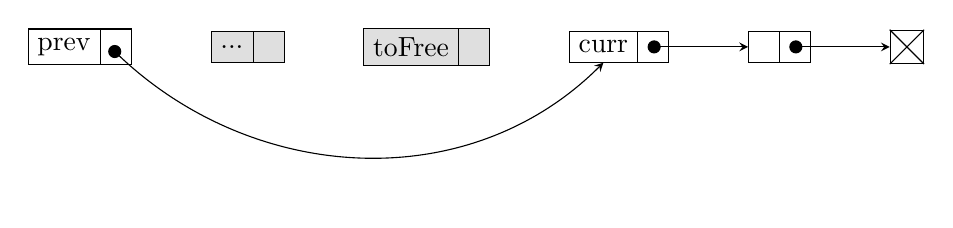
\begin{tikzpicture}[list/.style={rectangle split, rectangle split parts=2,
    draw, rectangle split horizontal}, >=stealth, start chain]

  \node[list,on chain] (A) {prev};
  \node[list,on chain, fill=gray!25] (B) {...};
  \node[list,on chain, fill=gray!25] (C) {toFree};
  \node[list,on chain] (D) {curr};
  \node[list,on chain] (E) {};      
  \node[on chain,draw,inner sep=6pt] (F) {};
  \draw (F.north east) -- (F.south west);
  \draw (F.north west) -- (F.south east);
  \draw[*->] let \p1 = (A.two), \p2 = (A.center) in (\x1,\y2) to[out=-45,in=-135] (D);
  \draw[*->] let \p1 = (D.two), \p2 = (D.center) in (\x1,\y2) -- (E);
  \draw[*->] let \p1 = (E.two), \p2 = (E.center) in (\x1,\y2) -- (F);  
\end{tikzpicture}
\end{center}

\begin{center}
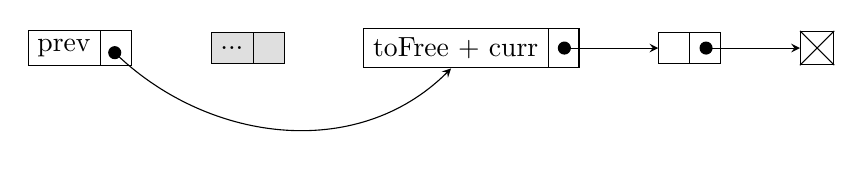
\begin{tikzpicture}[list/.style={rectangle split, rectangle split parts=2,
    draw, rectangle split horizontal}, >=stealth, start chain]

  \node[list,on chain] (A) {prev};
  \node[list,on chain, fill=gray!25] (B) {...};
  \node[list,on chain] (C) {toFree + curr};
  \node[list,on chain] (D) {};  
  \node[on chain,draw,inner sep=6pt] (E) {};
  \draw (E.north east) -- (E.south west);
  \draw (E.north west) -- (E.south east);
  \draw[*->] let \p1 = (A.two), \p2 = (A.center) in (\x1,\y2) to[out=-45,in=-135] (C);
  \draw[*->] let \p1 = (C.two), \p2 = (C.center) in (\x1,\y2) -- (D);  
  \draw[*->] let \p1 = (D.two), \p2 = (D.center) in (\x1,\y2) -- (E);
\end{tikzpicture}
\end{center}

We need to:
\begin{lstlisting}
Merge toFree + curr
prev.next = toFree
toFree.next = curr.next
\end{lstlisting}

Also, we don't want to merge with current if previous is at the end of the heap.

\item Chunk before toFree is free:

\begin{center}
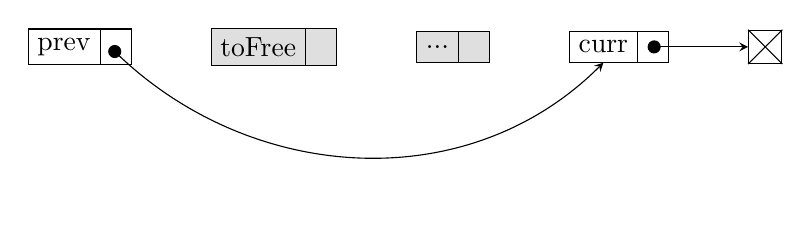
\begin{tikzpicture}[list/.style={rectangle split, rectangle split parts=2,
    draw, rectangle split horizontal}, >=stealth, start chain]

  \node[list,on chain] (A) {prev};
  \node[list,on chain, fill=gray!25] (B) {toFree};
  \node[list,on chain, fill=gray!25] (C) {...};
  \node[list,on chain] (D) {curr};    
  \node[on chain,draw,inner sep=6pt] (E) {};
  \draw (E.north east) -- (E.south west);
  \draw (E.north west) -- (E.south east);
  \draw[*->] let \p1 = (A.two), \p2 = (A.center) in (\x1,\y2) to[out=-45,in=-135] (D);
  \draw[*->] let \p1 = (D.two), \p2 = (D.center) in (\x1,\y2) -- (E);
\end{tikzpicture}
\end{center}

\begin{center}
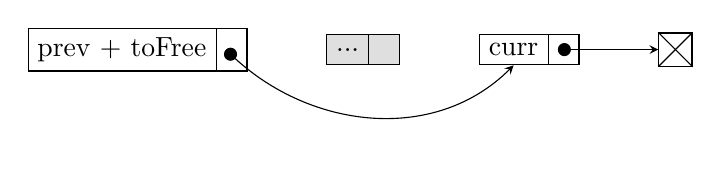
\begin{tikzpicture}[list/.style={rectangle split, rectangle split parts=2,
    draw, rectangle split horizontal}, >=stealth, start chain]

  \node[list,on chain] (A) {prev + toFree};
  \node[list,on chain, fill=gray!25] (B) {...};
  \node[list,on chain] (C) {curr};    
  \node[on chain,draw,inner sep=6pt] (D) {};
  \draw (D.north east) -- (D.south west);
  \draw (D.north west) -- (D.south east);
  \draw[*->] let \p1 = (A.two), \p2 = (A.center) in (\x1,\y2) to[out=-45,in=-135] (C);
  \draw[*->] let \p1 = (C.two), \p2 = (C.center) in (\x1,\y2) -- (D);  
\end{tikzpicture}
\end{center}

We need to:
\begin{lstlisting}
Merge prev + toFree
\end{lstlisting}

Also, we don't want to merge with the dummy head.

\item Chunks before and after toFree are free:

\begin{center}
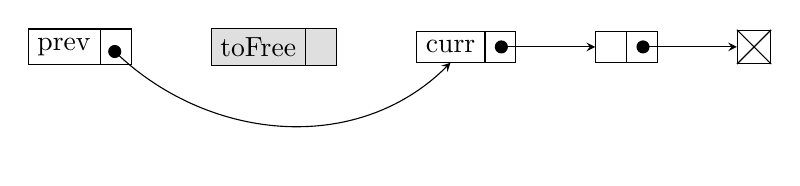
\begin{tikzpicture}[list/.style={rectangle split, rectangle split parts=2,
    draw, rectangle split horizontal}, >=stealth, start chain]

  \node[list,on chain] (A) {prev};
  \node[list,on chain, fill=gray!25] (B) {toFree};
  \node[list,on chain] (C) {curr};    
  \node[list,on chain] (D) {};    
  \node[on chain,draw,inner sep=6pt] (E) {};
  \draw (E.north east) -- (E.south west);
  \draw (E.north west) -- (E.south east);
  \draw[*->] let \p1 = (A.two), \p2 = (A.center) in (\x1,\y2) to[out=-45,in=-135] (C);
  \draw[*->] let \p1 = (C.two), \p2 = (C.center) in (\x1,\y2) -- (D);  
  \draw[*->] let \p1 = (D.two), \p2 = (D.center) in (\x1,\y2) -- (E);
\end{tikzpicture}
\end{center}

\begin{center}
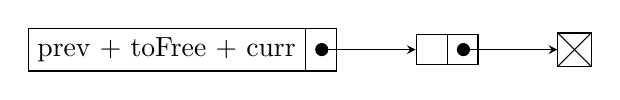
\begin{tikzpicture}[list/.style={rectangle split, rectangle split parts=2,
    draw, rectangle split horizontal}, >=stealth, start chain]

  \node[list,on chain] (A) {prev + toFree + curr};  
  \node[list,on chain] (B) {};    
  \node[on chain,draw,inner sep=6pt] (C) {};
  \draw (C.north east) -- (C.south west);
  \draw (C.north west) -- (C.south east);
  \draw[*->] let \p1 = (A.two), \p2 = (A.center) in (\x1,\y2) -- (B);
  \draw[*->] let \p1 = (B.two), \p2 = (B.center) in (\x1,\y2) -- (C);
\end{tikzpicture}
\end{center}

We need to:
\begin{lstlisting}
Merge prev + toFree + curr
prev.next = curr.next
\end{lstlisting}
This case is just an extension of sub case 2 and 3. However, if we applied sub case 2 and 3 (in that order), the prev chunk will be stuck pointing at toFree + curr chunk.\\

\begin{center}
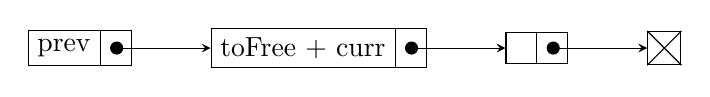
\begin{tikzpicture}[list/.style={rectangle split, rectangle split parts=2,
    draw, rectangle split horizontal}, >=stealth, start chain]

  \node[list,on chain] (A) {prev};
  \node[list,on chain] (B) {toFree + curr};
  \node[list,on chain] (C) {};  
  \node[on chain,draw,inner sep=6pt] (D) {};
  \draw (D.north east) -- (D.south west);
  \draw (D.north west) -- (D.south east);
  \draw[*->] let \p1 = (A.two), \p2 = (A.center) in (\x1,\y2) -- (B);
  \draw[*->] let \p1 = (B.two), \p2 = (B.center) in (\x1,\y2) -- (C);  
  \draw[*->] let \p1 = (C.two), \p2 = (C.center) in (\x1,\y2) -- (D);
\end{tikzpicture}
\end{center}

To fix this, we need to update sub case 3 to set: prev.next = toFree.next.

\begin{center}
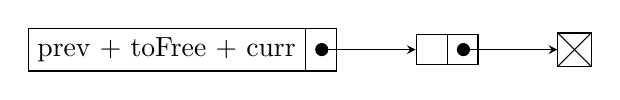
\begin{tikzpicture}[list/.style={rectangle split, rectangle split parts=2,
    draw, rectangle split horizontal}, >=stealth, start chain]

  \node[list,on chain] (A) {prev + toFree + curr};  
  \node[list,on chain] (B) {};    
  \node[on chain,draw,inner sep=6pt] (C) {};
  \draw (C.north east) -- (C.south west);
  \draw (C.north west) -- (C.south east);
  \draw[*->] let \p1 = (A.two), \p2 = (A.center) in (\x1,\y2) -- (B);
  \draw[*->] let \p1 = (B.two), \p2 = (B.center) in (\x1,\y2) -- (C);
\end{tikzpicture}
\end{center}

\item Sub case 3, Chunk before toFree is free (revised):

The solution for sub case 4 actually changes sub case 3 and adds a new line of code: prev.next = toFree.next. We need to make sure it still works. What happens if sub case 2 does not occur (i.e. we don't merge with current)? Then we set toFree.next = current, as a part of sub case 1.

\begin{center}
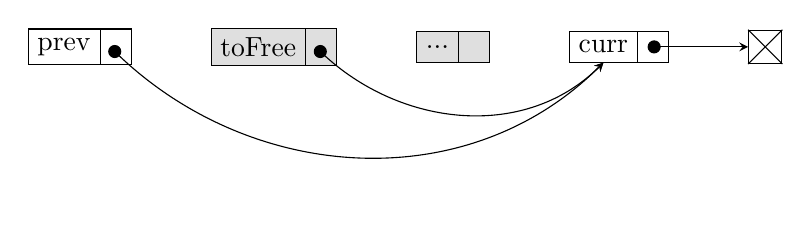
\begin{tikzpicture}[list/.style={rectangle split, rectangle split parts=2,
    draw, rectangle split horizontal}, >=stealth, start chain]

  \node[list,on chain] (A) {prev};
  \node[list,on chain, fill=gray!25] (B) {toFree};
  \node[list,on chain, fill=gray!25] (C) {...};
  \node[list,on chain] (D) {curr};    
  \node[on chain,draw,inner sep=6pt] (E) {};
  \draw (E.north east) -- (E.south west);
  \draw (E.north west) -- (E.south east);
  \draw[*->] let \p1 = (A.two), \p2 = (A.center) in (\x1,\y2) to[out=-45,in=-135] (D);
  \draw[*->] let \p1 = (B.two), \p2 = (B.center) in (\x1,\y2) to[out=-45,in=-135] (D);  
  \draw[*->] let \p1 = (D.two), \p2 = (D.center) in (\x1,\y2) -- (E);
\end{tikzpicture}
\end{center}

Then, if sub case 3 occurs, we merge prev and toFree and do prev.next = toFree.next which does not change sub case 3.

\begin{center}
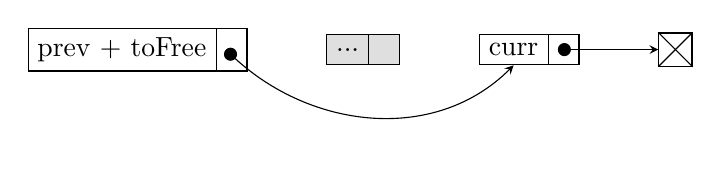
\begin{tikzpicture}[list/.style={rectangle split, rectangle split parts=2,
    draw, rectangle split horizontal}, >=stealth, start chain]

  \node[list,on chain] (A) {prev + toFree};
  \node[list,on chain, fill=gray!25] (B) {...};
  \node[list,on chain] (C) {curr};    
  \node[on chain,draw,inner sep=6pt] (D) {};
  \draw (D.north east) -- (D.south west);
  \draw (D.north west) -- (D.south east);
  \draw[*->] let \p1 = (A.two), \p2 = (A.center) in (\x1,\y2) to[out=-45,in=-135] (C);
  \draw[*->] let \p1 = (C.two), \p2 = (C.center) in (\x1,\y2) -- (D);  
\end{tikzpicture}
\end{center}

\end{enumerate}

\begin{lstlisting}
def free(toFree) = {
	def find(prev) = {
		val current = next(prev)
		
		if (current < toFree){
			find(current)
		} else {
			// Case 2, check if we can merge with current
			if (toFree + size(toFree) == current && 
					current < heapStart + heapSize){
				setSize(toFree, size(toFree) + size(current))
				setNext(prev, toFree)
				setNext(toFree, next(current))
			} else {
				setNext(toFree, current)
			}
			
			// Case 3, check if we can merge with previous
			if (prev + size(prev) == toFree && 
					prev > heapStart){
				setSize(prev, size(prev) + size(toFree)
				// Required for case 4 to work
				setNext(prev, next(toFree))
			} else {
				setNext(prev, toFree)
			}
		}
	}
	
	find(heapStart)
}
\end{lstlisting}

What is the running time of this heap data structure?

Allocation: \(O(\vert heap \vert)\). Deallocation: \(O(\vert heap \vert)\).\\

Note that we could improve the algorithm for deallocation to \(O(1)\) if we had access to more memory and used a doubly linked list.

\subsubsection{Fragmentation}
E.g. Consider the following code:

\begin{minipage}[t]{0.5\textwidth}
\begin{lstlisting}
a = malloc(8)
b = malloc(8)
c = malloc(8)
free(a)
free(b)
\end{lstlisting}
\end{minipage}
\begin{minipage}[t]{0.5\textwidth}
\begin{center}

\begin{minipage}[t]{0.25\textwidth}
Heap

\begin{tabular}{|c|}
\hline
a\\
\hline
b\\
\hline
c\\
\hline
\end{tabular}
\end{minipage}
\begin{minipage}[t]{0.25\textwidth}
Heap

\begin{tabular}{|c|}
\hline
\\
\\
\hline
c\\
\hline
\end{tabular}
\end{minipage}
\end{center}
\end{minipage}\\
Then a and b will be merged into one free chunk.\\

E.g. Consider the following code:

\begin{minipage}[t]{0.5\textwidth}
\begin{lstlisting}
a = malloc(8)
b = malloc(8)
c = malloc(8)
free(a)
free(c)
\end{lstlisting}
\end{minipage}
\begin{minipage}[t]{0.5\textwidth}
\begin{center}

\begin{minipage}[t]{0.25\textwidth}
Heap

\begin{tabular}{|c|}
\hline
a\\
\hline
b\\
\hline
c\\
\hline
\end{tabular}
\end{minipage}
\begin{minipage}[t]{0.25\textwidth}
Heap

\begin{tabular}{|c|}
\hline
\\
\hline
b\\
\hline
\\
\hline
\end{tabular}
\end{minipage}
\end{center}
\end{minipage}\\
No chunk will be merged.\\

Notice that the two examples result in the exact same amount of memory, 8 bytes. However, in the second example, we cannot allocate a chunk of size 8.\\

This problem is called fragmentation. A heap is fragmented when it is split into many small pieces. Fragmentation can cause out of memory errors even when most of the heap is free.\\

Defragmentation (also called compacting) is the process of moving all used chunks in memory and putting them at the beginning of the heap. Compaction needs to update all pointers in the program so they point to their new locations.\\

How can we update all pointers in the program?

First we need to know where the pointers actually are. The only way can know this is through a sound type system. Recall the Lacs type system is sound and there are two types, Integers and Function values, where the latter is a pointer.\\

Convention: A chunk will look like the following:
\begin{center}
\begin{tabular}{|c|}
\hline
Size\\
\hline
Number of pointers\\
\hline
Pointers\\
..\\
\hline
Non-pointers\\
..\\
\hline
\end{tabular}
\end{center}

A chunk is live if it will be read later in the program. We need to move all lives chunk to the beginning of the heap. How do we determine which chunks are live? We could let the programmer tell us (like in C/C++). However, it would be nice if we could somehow predict which chunks are live, even if it is an approximation. We will apply the concept of reachable chunks to approximate live chunks.\\

A chunk is reachable if:
\begin{itemize}
\item Its address is stored in the stack or register
\item Its address is stored in another reachable chunk
\end{itemize}

In general, if a chunk is live then it is reachable. However the converse is not always true. There could be chunks that are reachable but dead. Remember that the concept of reachable chunks is only an approximation to live chunks.\\

Lets study an algorithm that applies the concept of reachable chunks to a automatic garbage collector.

\subsubsection{Cheney's Garbage Collector}
Main idea: split the heap into two halves called semispaces. The first half is called the from-space and the second half is called the to-space. Always allocate in the from-space. When the from-space is full, perform compaction and move all reachable chunks to the to-space. Then switch the from-space and to-space.\\

Convention: The from-space and to-space will take 25\% of heapSize. The from-space will start as the first half. The heapPtr register points to one word after the end of the used heap space. That is, everything about the heapPtr is used space. The variable "semiSpaceTop" will point to one word after the end of from-space. \\

\begin{center}
\begin{tabular}{|c|}
\hline
Code\\
..\\
\hline
From-space\\
..\\
\hline
To-space\\
..\\
\hline
Stack\\
..\\
\hline
\end{tabular}
\end{center}

\begin{lstlisting}
def init() = {
	heapPtr = heapStart
	semiSpaceTop = heapMiddle
}

def allocate(wanted) = {
	if (heapPtr + wanted > semiSpaceTop){
		gc()
	}
	
	val ret = heapPtr
	heapPtr = heapPtr + wanted
	ret
}
\end{lstlisting}
Note that if semiSpaceTop is equal to heapPtr + wanted, then the from-space would be exactly full after allocating a chunk of size wanted. The next time we allocate a chunk we'll need to call the garbage collector and perform compaction.\\

The main algorithm is as follows:
\begin{enumerate}
\item First we need to find all the reachable chunks from the stack. To do this, we go through all chunks in the stack. If any of these chunks have pointer variables, we check to see if they point to chunks in the from-space. If they do, we check to see if the chunk has already been copied. If so, just return the new address. If not, we copy the chunk from the from-space to the to-space and return the new address of the chunk. Then we need to update the pointer so it pointers to the new location of the chunk.

\item After we are done scanning the stack, the to-space will be filled with a bunch of chunks that are reachable from the stack. Now we need to scan each of those chunks to see if any of them contain pointers to chunks in the from-space. If they do, then that chunk is also reachable since it has a pointer from a reachable chunk. We copy the chunk from the from-space to the to-space and update the pointer so it pointers to the new address.

\item After we are done scanning all the chunks in the to-space, we will have processed every reachable chunk in memory. Now we update the heapPtr = free and then switch the from-space and to-space.
\end{enumerate}

Note that Cheney's algorithm actually uses the to-space as a queue. At first, the to-space holds all the reachable chunks from the stack. Then, as we process each of those reachable chunks, more reachable chunks get pushed onto the to-space for us to process later. We will eventually be done processing all chunks in the to-space because there are finitely many reachable chunks in memory.\\

\begin{lstlisting}[escapeinside={(*}{*)}]
def gc() = {
	val toSpace = if (semiSpaceTop == heapMiddle) heapMiddle else heapStart
	val free = toSpace
	
	// Start scanning from top of the stack excluding gc's frame
	var scan = gc.dynamicLink
	while (scan < memSize){
		forwardPtrs(scan)
		scan = scan + size(scan)
	}
	
	scan = toSpace
	while (scan < free){
		forwardPtrs(scan)
		scan = scan + size(scan)
	}
	
	semiSpaceTop = toSpace + semiSpaceSize
	heapPtr = free
}

def forwardPtrs(chunk){
	for each offset o that holds a pointers {
		val newAddress = copy(deref(chunk + o))
		assignToAddress(chunk + o, newAddress)
	}
}

def copy(chunk){
	if (chunk not in from-space){
		chunk
	} else {
		if (size(chunk) (*$\geq$*) 0){
			copyChunk(free, chunk)
			setSize(chunk, -size(chunk))
			setNext(chunk, free)
			free = free + size(free)
		}
		
		next(chunk)
	}
}
\end{lstlisting}

Note: forwardPtrs and copy should be nested procedures of gc. When implementing the algorithm on the assignments, make sure that the procedure that calls gc() has its frame on the stack (and not the heap). When a chunk is copied to the to-space, we negate its size to indicate that it has been copied. We store the address that the chunk has been copied to in the second word of the chunk.\\

\newpage

E.g. Run Cheney's algorithm on the following code:\\

\begin{minipage}[t]{0.5\textwidth}
\begin{lstlisting}
forwardPtrs(120) // No Ptrs
\end{lstlisting}
\begin{lstlisting}
forwardPtrs(132) // Ptrs: 8
\end{lstlisting}
	\begin{itemize}
		\item copy(deref(132 + 8)) \(\rightarrow\) copy(36)
		\begin{itemize}
			\item 36 is in from-space
			\item copyChunk(72, 36)
			\item setSize(36, -12)
			\item setNext(36, 72)
			\item Return 72
		\end{itemize}		
		\item assignToAddr(132 + 8, 72)
	\end{itemize}
\begin{lstlisting}
forwardPtrs(72) // Ptrs: 8
\end{lstlisting}
	\begin{itemize}
		\item copy(deref(72 + 8)) \(\rightarrow\) copy(48)
			\begin{itemize}
				\item 48 is in from-space
				\item copyChunk(84, 48)
				\item setSize(48, -12)
				\item setNext(48, 84)
				\item Return 84
			\end{itemize}
		\item assignToAddr(72 + 8, 84)
	\end{itemize}
\begin{lstlisting}
forwardPtrs(84) // Ptrs: 8
\end{lstlisting}
	\begin{itemize}
		\item copy(deref(84 + 8)) \(\rightarrow\) copy(36)
			\begin{itemize}
				\item 36 is in from-space
				\item 36 has already been copied
				\item Return 72
			\end{itemize}
		\item assignToAddr(84 + 8, 72)	
	\end{itemize}
\end{minipage}
\begin{minipage}[t]{0.5\textwidth}
	\begin{center}
		From-space\\
		\begin{tabular}{|c|c|}
			\hline
			36 & size = 12 \(\rightarrow\) -12\\
			\hline
			40 & ptrs = 1 \(\rightarrow\) 72\\
			\hline
			44 & 48\\
			\hline
			48 & size = 12 \(\rightarrow\) -12\\
			\hline
			52 & ptrs = 1 \(\rightarrow\) 84\\
			\hline
			56 & 36\\
			\hline
			60 & \\
			\hline			
			64 & \\
			\hline			
			68 & \\
			\hline
		\end{tabular}
		
		\vspace{7mm}
		
		To-space\\
		\begin{tabular}{|c|c|}
			\hline
			72 & size = 12 \\
			\hline
			76 & ptrs = 1 \\
			\hline
			80 & 48 \(\rightarrow\) 84 \\
			\hline
			84 & size = 12\\
			\hline
			88 & ptrs = 1 \\
			\hline
			92 & 36 \(\rightarrow\) 72\\
			\hline
			96 & \\
			\hline			
			100 & \\
			\hline			
			104 & \\
			\hline
		\end{tabular}
		
		\vspace{7mm}
		
		Stack\\
		\begin{tabular}{|c|c|}
			\hline
			108 & \\
			\hline			
			112 & \\
			\hline			
			116 & \\
			\hline			
			120 & size = 12 \\
			\hline
			124 & ptrs = 0 \\
			\hline
			128 & 60 \\
			\hline
			132 & size = 12 \\
			\hline
			136 & ptrs = 1 \\
			\hline
			140 & 36 \(\rightarrow\) 72 \\
			\hline
		\end{tabular}				
	\end{center}
\end{minipage}

What is the running time of Cheney's garbage collector?

Allocation: Best case: \(\Omega(1)\). Worst case: \(O(\vert \text{reachable chunks} \vert)\).\\

The major disadvantage of the algorithm is that it wastes 25\% of memory. Real life compilers use generational garbage collection. Generational garbage collection observes that most memory either dies young or lives long. Instead of having only 2 semispaces there are multiple semispaces. There are small-sized semispaces for short lived memory where the garbage collector runs frequently. There are large-sized semispaces for long lived memory where the garbage collector runs infrequently.\\

How do they determine short lived memory and long lived memory?

They approximate. All chunks that still exist after 100 garbage collector runs is probably long lived memory. This can get very complex because all these different semispaces can have pointers between each other and we need another data structure to keep track of that.

\newpage

\section{Lambda Calculus}
Lambda calculus is a theoretical mathematical model of programs. All calculations are done through a context free grammar:\\

e \(\rightarrow\) v (i.e. An expression is a variable)\\
e \(\rightarrow\) e e (i.e. An expression is a function call. The left e evaluates to a function/closure and the right e are the arguments) \\
e \(\rightarrow\) \(\lambda\) v. e (An expression is a function declaration. The function has parameter v and function body e)\\

Just like there is a step function for MIPs assembly, there is a step function for lambda calculus called \(\beta\)-reduction:\\

(\(\lambda\) v. \(e_1\)) \(e_2\) \(\rightarrow\) \(e_1\)[\(e_2\)/v] (i.e. Evaluates to \(e_1\) with \(e_2\) replacing v in the function body)\\

E.g. (\(\lambda\) v. v v)(a b c) \(\rightarrow\) (a b c)(a b c)\\

E.g. (\(\lambda\) v. v v)(\(\lambda\) x. x x) \(\rightarrow\) (\(\lambda\) x. x x)(\(\lambda\) x. x x) \(\rightarrow\) (\(\lambda\) x. x x)(\(\lambda\) x. x x) \(\rightarrow\) (\(\lambda\) x. x x)(\(\lambda\) x. x x)... There can be infinite loops in lambda calculus.\\

E.g. \(\lambda\) y. ((\(\lambda\) x. (\(\lambda\) y. x)  y) y)\\

Notice that inside the main function body, y evaluates to the global y. But inside the middle function body, y evaluates to a local y. However, we cannot distinguish between the two y. This will cause a name clash so lets rename the inner y to y'.\\

=  \(\lambda\) y. ((\(\lambda\) x. (\(\lambda\) y'. x)  y) y) \(\rightarrow\) 
\(\lambda\) y. ((\(\lambda\) y'. y) y)
\end{document}